\section{Coastal Geomorphology}
\label{sec:coastal_geomorphology}

The Portuguese coast presents high tsunami inundation risk in comparison with other locations of the Atlantic Europe due to its close location in relation to the Azores-Gibraltar plate boundary.
The Portuguese coastline presents several high-energy sedimentary deposits\footnote{Typically associated with intense wave activity, promoting resuspension and transport of larger particles.} associated with onshore depositional activity from the AD 1755 Lisbon event, with both large and small boulders located above mean sea level and occurring between Lisbon and the central Algarve attributed to deposition by this and older tsunamis \citep{Scheffers-2005, Costa-2008}. Furthermore, the western Portuguese coast is also very exposed to Atlantic storms, and wave power associated with wind-generated waves is also very high \citep{Oliveira-2011}. 

Such characteristics make the western coast of Portugal an important study area regarding entrainment and transport of large clasts (including megaclasts) by storm or tsunami waves, a matter that has been profusely discussed in the literature in the last decade. Although the exact mechanism that originates such deposits still lacks an exact comprehension, several authors used conventional numerical solutions that simulate particle transport, sometimes with contradictory results \citep{Nandasena-2011, Kain-2012}. The biggest challenge has been the differentiation of the events (storm or tsunami), and the reconstruction of wave parameters (e.g. wave height, length, direction) responsible for the entrainment and transport of these megaclasts. Conceptual efforts have been made to distinguish between the two, with the most popular approach being \cite{Nott-2003} methodology, that attempts to differentiate the two origins in a variety of dynamic and geological environments, but disregarding local features.

A practical example of such phenomena can be observed in Praia das Ma\c{c}\~{a}s, Portugal. The location is a pocket beach encased in a high energy exposed cliffed coast. The geology consists of Cretaceous soft marls alternated with resistant limestone. A seaward sloping close to $80$ m wide stepped rock platform develops at the cliff toe. The step characteristics are controlled by practically vertical fractures and the thickness of the resistant limestone layers, typically close to $1$ m. In Figure \ref{fig:boulders_exp}, two boulders that suffered transport are identified.

%
\begin{figure}[ht!]
	\centering
	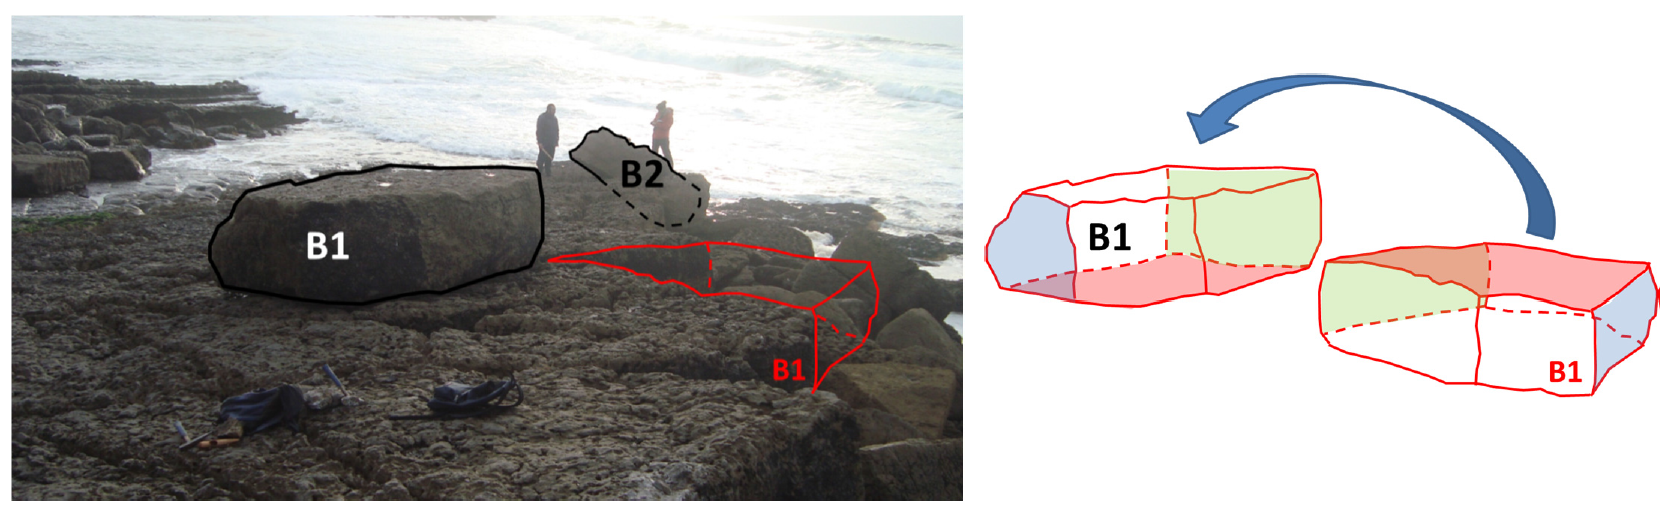
\includegraphics[width=0.85\linewidth]{Figures/6.Chapter/boulders_exp} 
	\caption{Praia das Ma\c{c}\~{a}s, Portugal. Boulder identification and orientation. \cite{Oliveira-2011}}
	\label{fig:boulders_exp} 
\end{figure}
%

Boulder B1 is $2.80\times2.0\times1.0$ m and weighs approximately 14 ton. It appears to have suffered a rotation and a small translation from the initial position. In this exploratory Section, the proposed model is applied as an inverse-problem, attempting to reproduce the dislodgement of megaclast, i.e, it is hypothesized that the pattern of deposition may be partially explained by actually modeling specific events in real geometries, attempting to recover the final observed state. 

The geometry of the problem is idealized but represents the key features of the overhanging layers related with fractures, bedding and differential erosion of sub-horizontal layers that originated block B1. In plan view, concave and convex coastline shapes are tested to assess the influence of momentum accumulation. A paddle with prescribed motion was used to generate a wave with $40\;m$ wavelength and $15\;m$ height, reproducing a large storm wave that breaks at the beach section. The lateral dimension is periodic to avoid any wall effects and the $2.84\times10^6$ particles are a result of $Dp=0.10\;m$ resolution, forcing 13 h long computations for 25 s events. The megaclast is assumed to be homogeneous limestone, with $E=4.5\times10^8 Nm^{-2}$, $\nu=0.15$ and $\mu=0.60$. Figures \ref{fig:boulders_I} to \ref{fig:boulders_IV} show the evolution of the system as the wave impacts the overhanging boulder.

%
\begin{figure}[ht!]
	\centering
	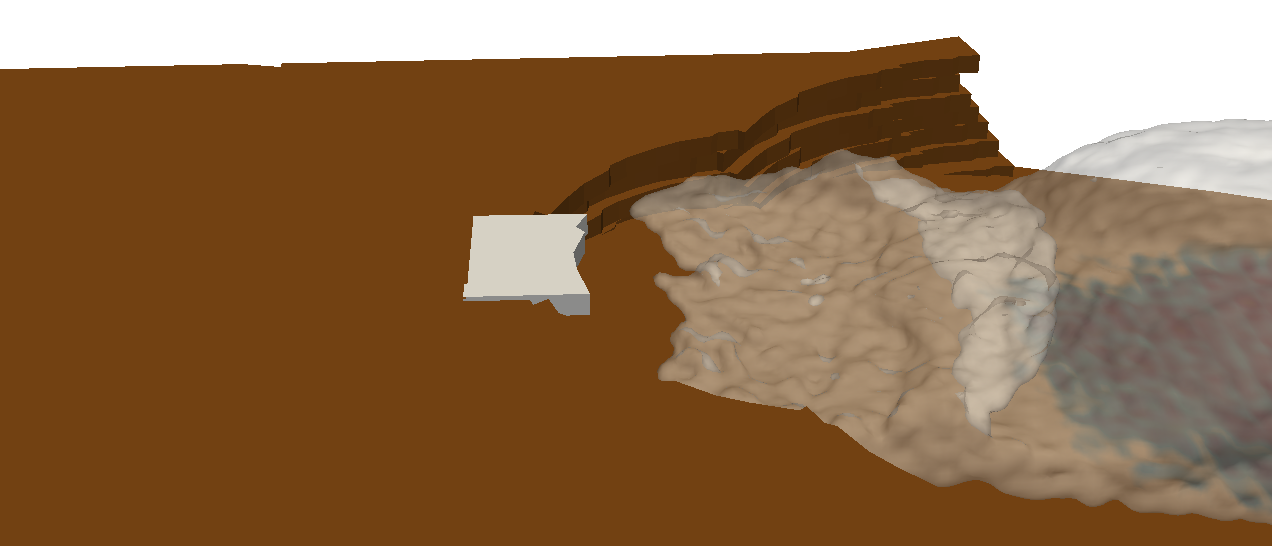
\includegraphics[width=0.42\linewidth]{Figures/6.Chapter/concave_105} 
	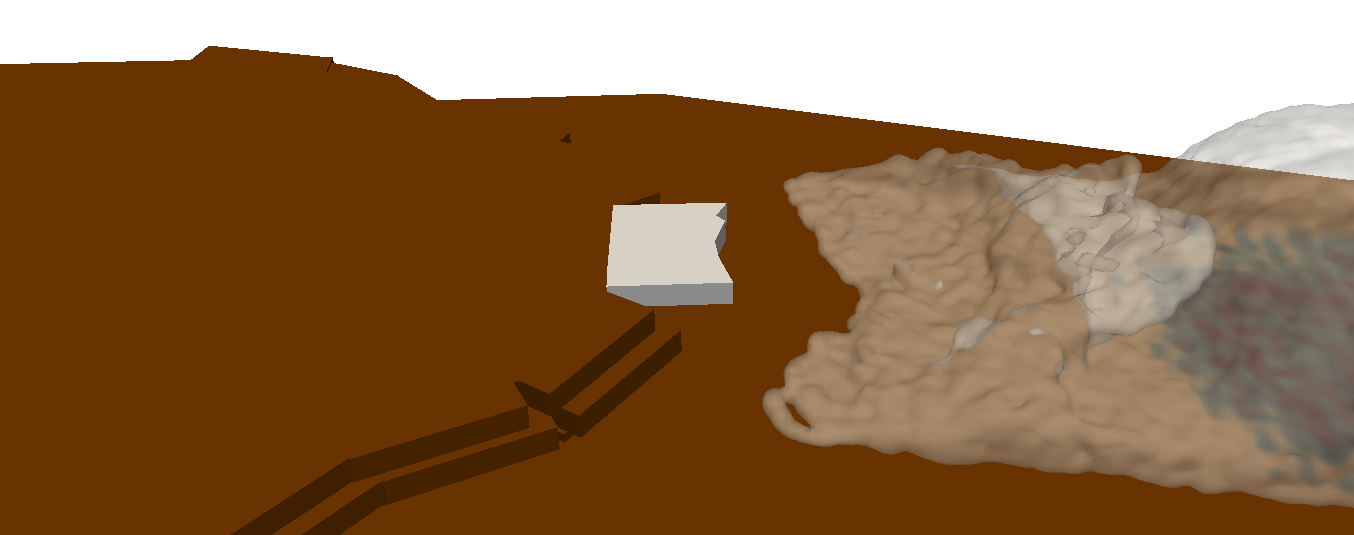
\includegraphics[width=0.42\linewidth]{Figures/6.Chapter/convex_105}
	%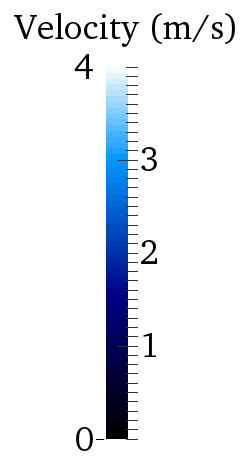
\includegraphics[width=0.13\linewidth]{Figures/6.Chapter/label} 
	\caption{Concave and convex geometries, $t=10.5$ s.}
	\label{fig:boulders_I} 
\end{figure}
%

%
\begin{figure}[ht!]
	\centering
	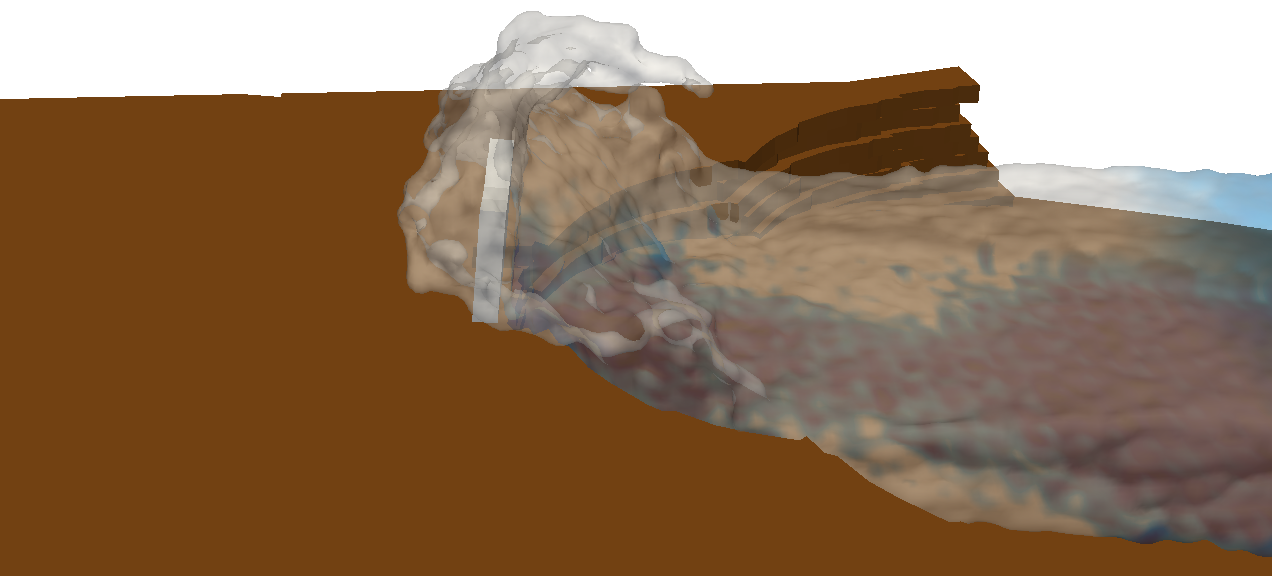
\includegraphics[width=0.42\linewidth]{Figures/6.Chapter/concave_115} 
	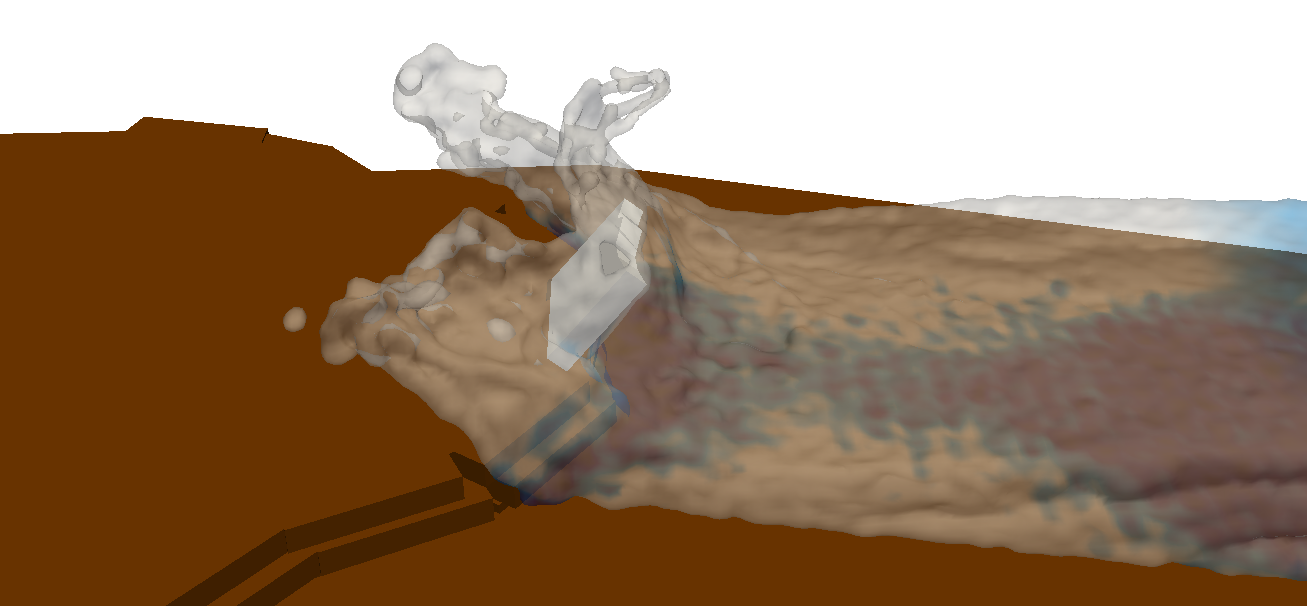
\includegraphics[width=0.42\linewidth]{Figures/6.Chapter/convex_115} 
	%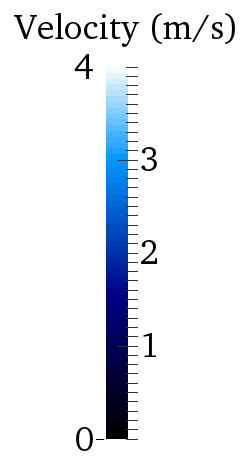
\includegraphics[width=0.13\linewidth]{Figures/6.Chapter/label} 
	\caption{Concave and convex geometries, $t=11.5$ s.}
	\label{fig:boulders_II} 
\end{figure}
%

%
\begin{figure}[ht!]
	\centering
	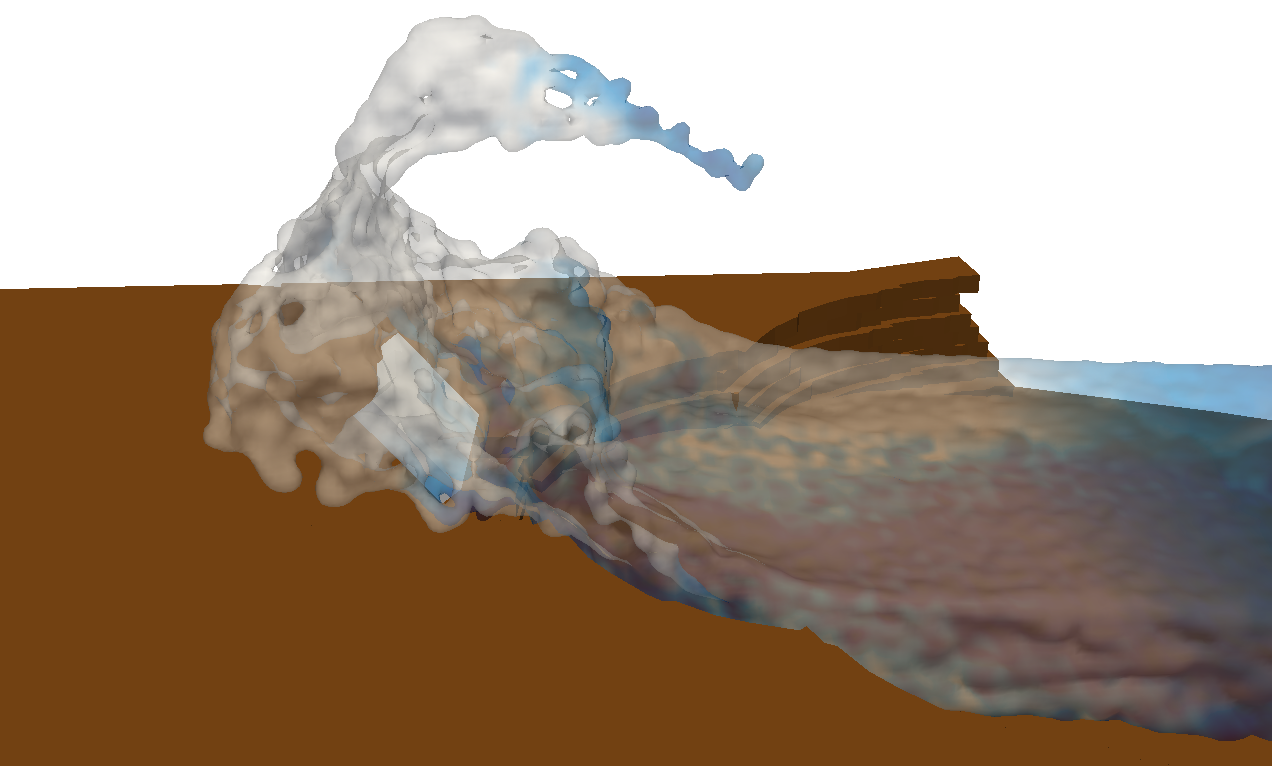
\includegraphics[width=0.42\linewidth]{Figures/6.Chapter/concave_120} 
	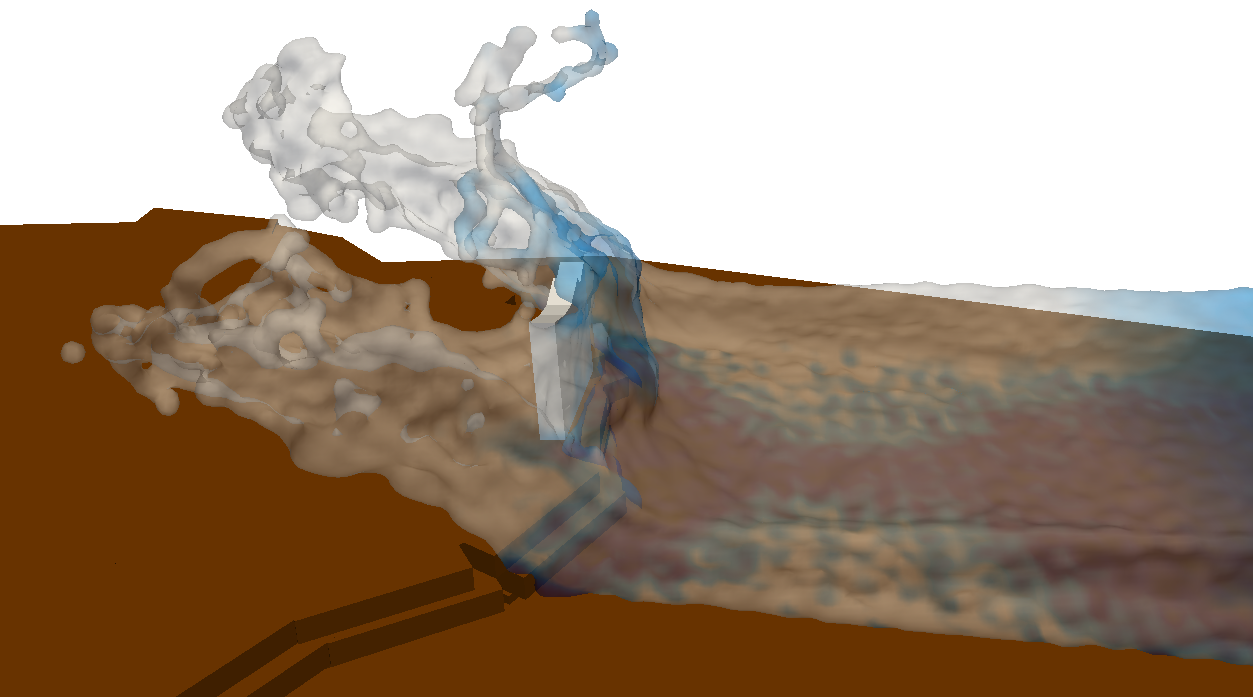
\includegraphics[width=0.42\linewidth]{Figures/6.Chapter/convex_120} 
	%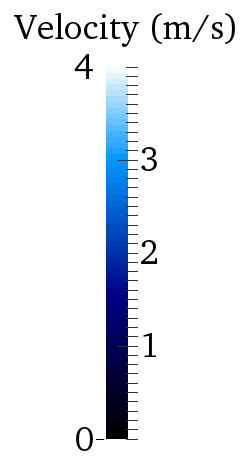
\includegraphics[width=0.13\linewidth]{Figures/6.Chapter/label} 
	\caption{Concave and convex geometries, $t=12.0$ s.}
	\label{fig:boulders_III} 
\end{figure}
%

%
\begin{figure}[ht!]
	\centering
	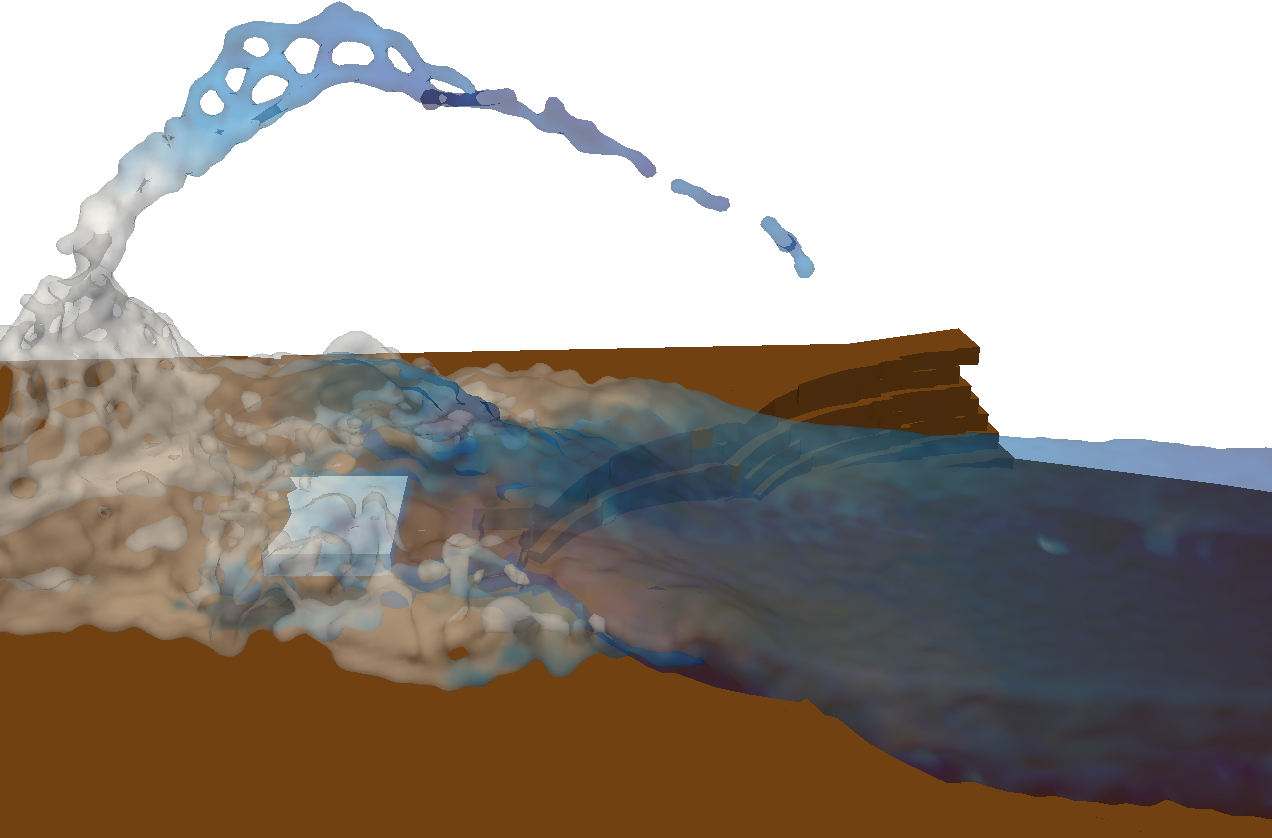
\includegraphics[width=0.42\linewidth]{Figures/6.Chapter/concave_130} 
	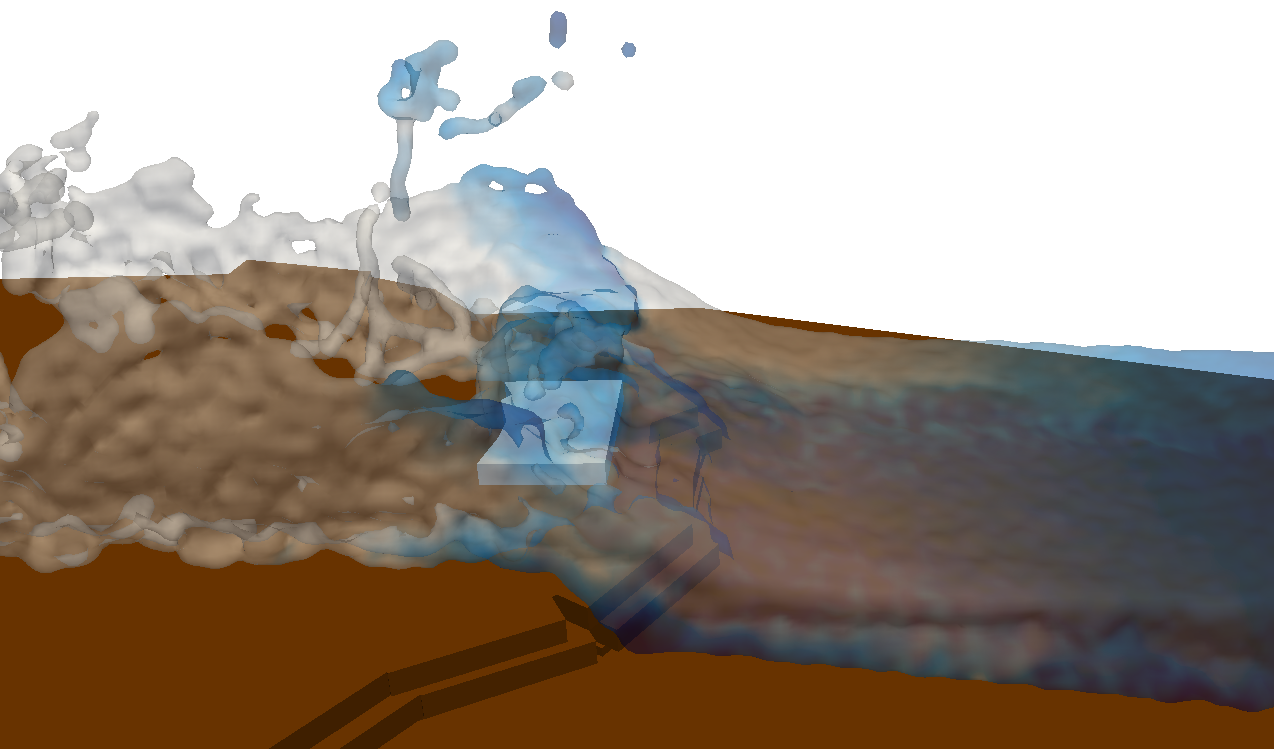
\includegraphics[width=0.42\linewidth]{Figures/6.Chapter/convex_130} 
	%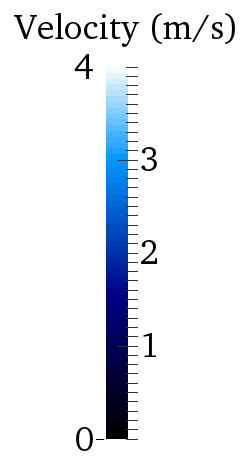
\includegraphics[width=0.13\linewidth]{Figures/6.Chapter/label} 
	\caption{Concave and convex geometries, $t=13.0$ s.}
	\label{fig:boulders_IV} 
\end{figure}
%

Differences in concave to convex geometries are within expectation: momentum seems to be concentrated in the concave case, as the megaclast rotates faster (Figure \ref{fig:boulders_III}) and is transported around $1$ m further comparing to the convex case. 

Another fundamental aspect of the phenomenon is overhanging versus supported geometry. Two contact forces are responsible for the dislodgement of the boulders: pressure and momentum flux. The main working force is the momentum flux, but the work of both for the boulder movement is proportional to the area exposed. Figures \ref{fig:boulders_V} and \ref{fig:boulders_VI} show the pressure field on the impact locus. 

%
\begin{figure}[ht!]
	\centering
	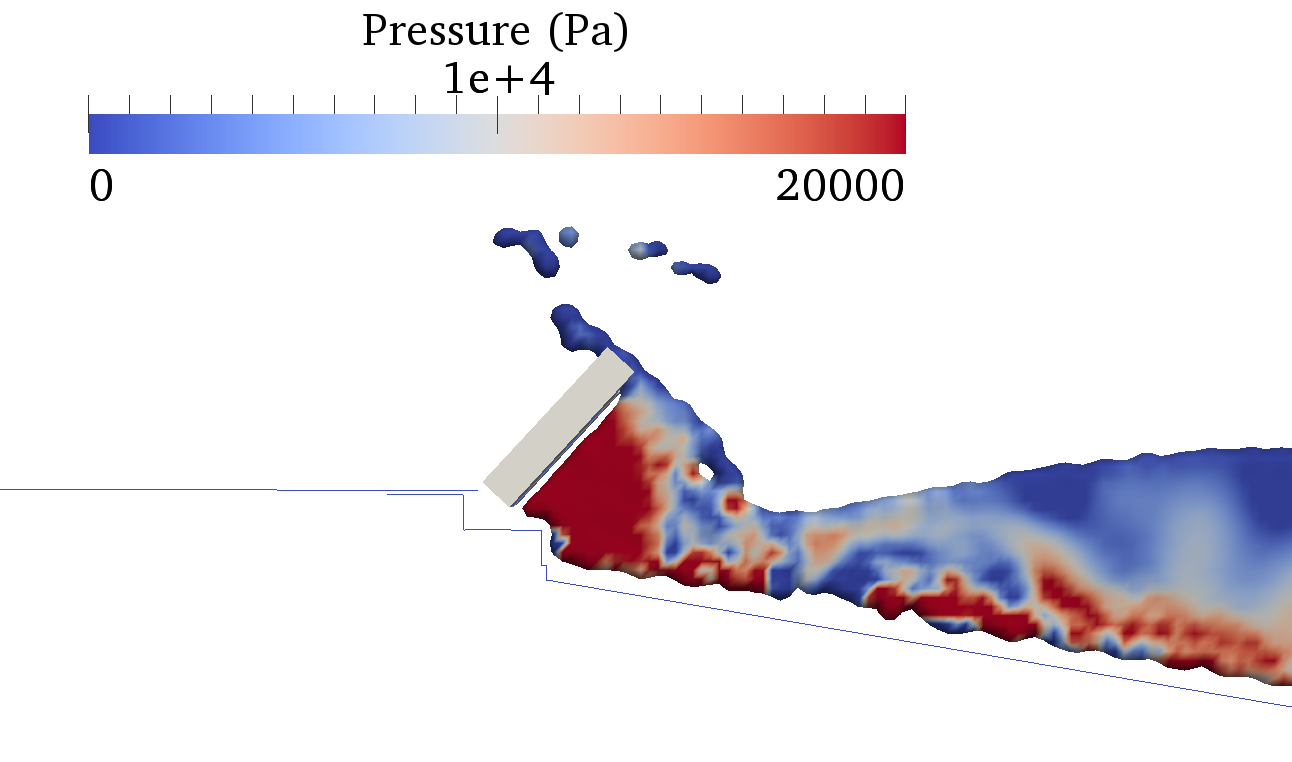
\includegraphics[width=0.48\linewidth]{Figures/6.Chapter/2D_press_norm_I} 
	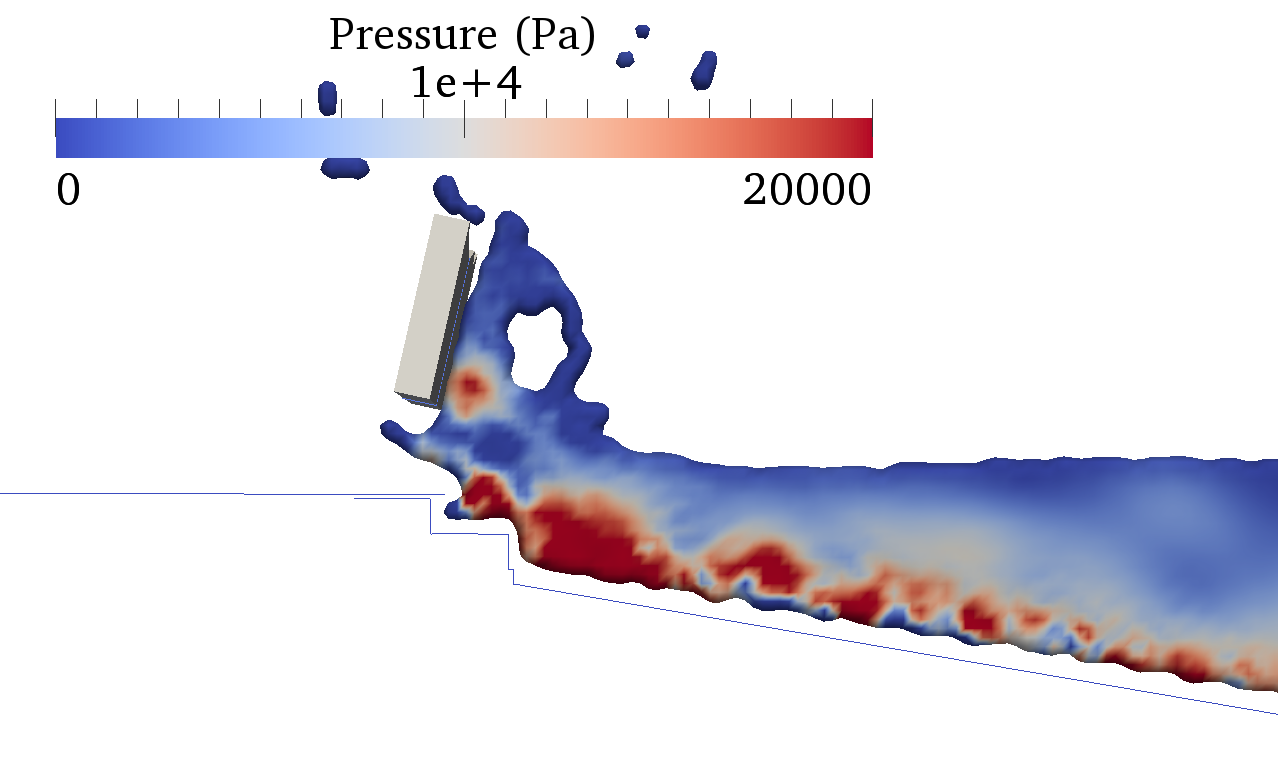
\includegraphics[width=0.48\linewidth]{Figures/6.Chapter/2D_press_norm_II}
	\caption{Concave geometry. Vertical plane over domain axis. Overhanging case. Left-$t=10.9$ s, right-$t=11.5$ s.}
	\label{fig:boulders_V} 
\end{figure}
%

%
\begin{figure}[ht!]
	\centering
	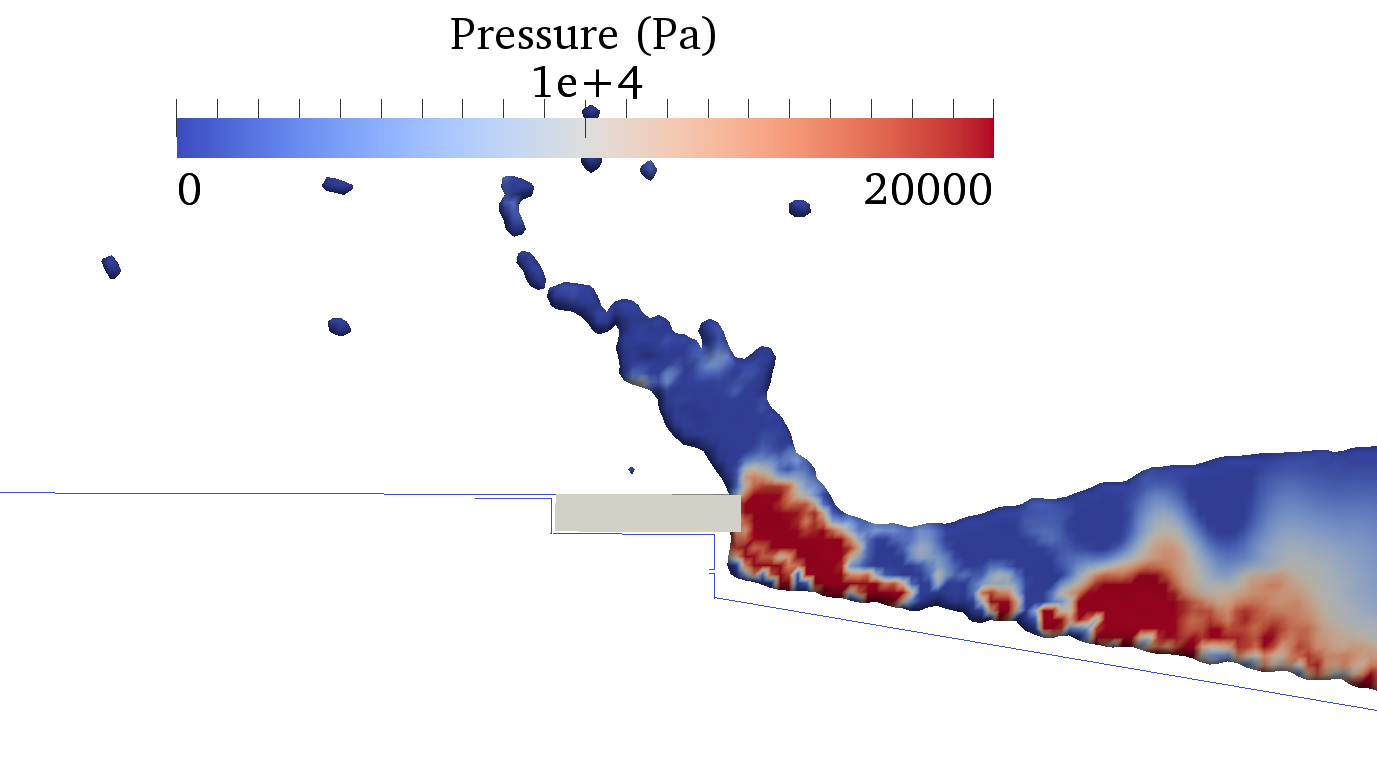
\includegraphics[width=0.48\linewidth]{Figures/6.Chapter/2D_press_flat}
	\caption{Concave geometry. Vertical plane over domain axis. Supported case. $t=11.5$ s.}
	\label{fig:boulders_VI} 
\end{figure}
%

As expected, a significant pressure build-up occurs in the impact locus. The cavity in the overhanging configuration allows the contact forces to produce work on the boulder, in contrast with the supported case.

The local (micro to meso-scale) geomorphological conditions in rocky coastal contexts strongly control the capability of waves to entrain and transport large particles upward and inland. The flow modulation induced by these features is not adequately addressed by conventional numerical solutions and requires the application of models capable of explicitly resolving the momentum transfer between phases and take into account complex geometrical considerations.





%%%%%%%%%%%%%%%%%%%%%%%%%%%%%%%%%%%%%%%%%%%%%%%%%%%%%%%%%%%
\section{Sines Port}
\label{sec:sines}

The Sines Container Terminal, called Terminal XXI, is a major infrastructure in the Portuguese coast, currently capable of handling 1,100,000 TEU, with plans of extending up to 1,700,000 TEU. As mentioned in Section \ref{sec:coastal_geomorphology} Portugal's Atlantic coast, especially southwards of Lisbon, is subject to a non negligible risk of tsunami waves caused by seismic events that occur offshore. These results show the influence of a wave in stacked containers and other obstacles in a reduced subsection of the quay, detailed in Figure \ref{fig:sines_map}.

%
\begin{figure}[ht!]
	\centering
	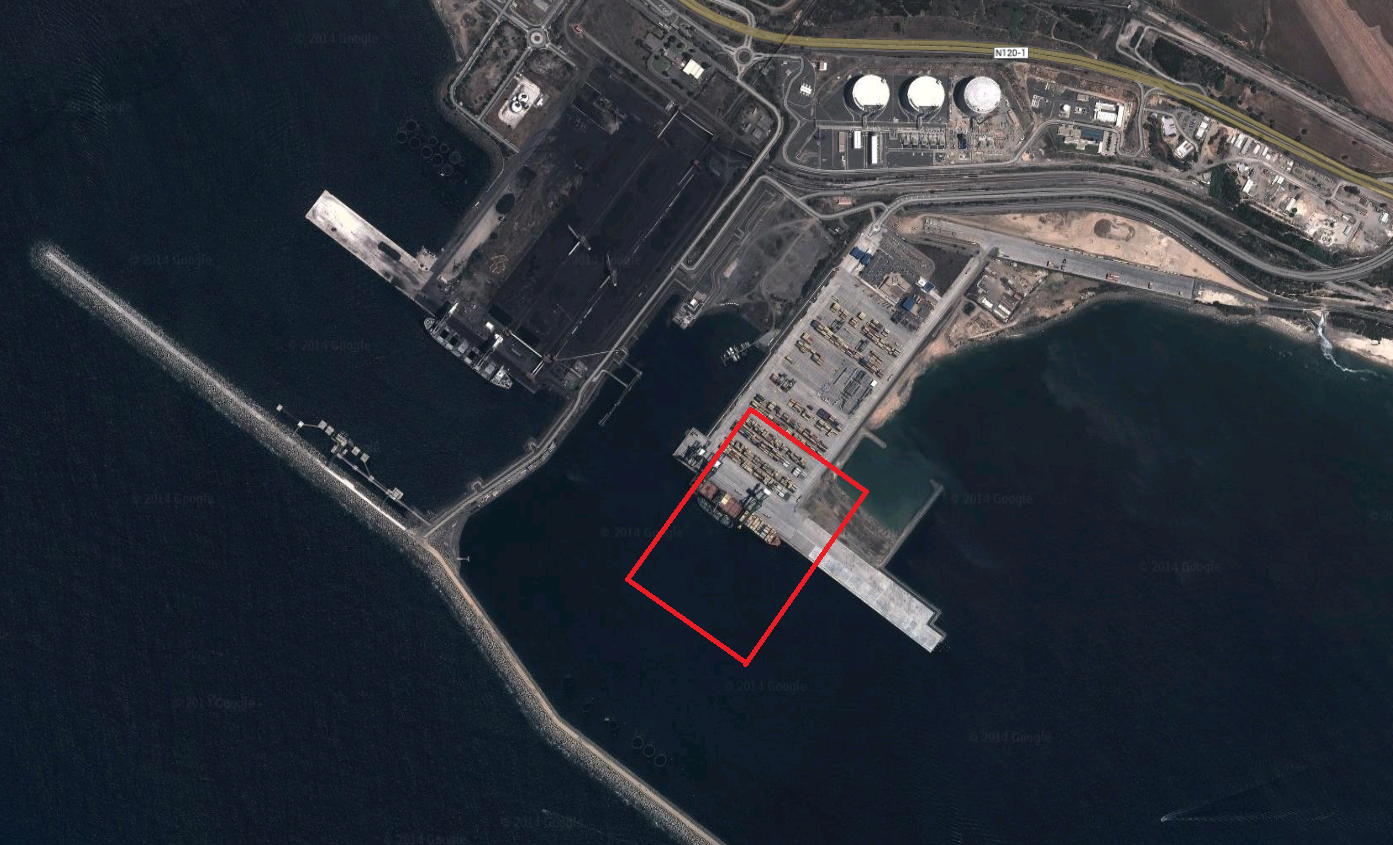
\includegraphics[width=0.80\linewidth]{Figures/6.Chapter/map_sines_domain} 
	\caption{Aerial view of the Terminal XXI of the Sines Port. Red square indicates the computational domain.}
	\label{fig:sines_map} 
\end{figure}
%

The section of the harbor is partially protected by a breakwater to the east, neglected in this case to simplify the behavior of the wave on the area of interest. The chosen domain originates an excess of $12\times10^6$ particles, for a $Dp=0.5$ m, resulting in a 57 h long computation for the 60 s event. The type of wave to be generated must observe some limitations, since the wavelength must be less than the domain extent, to avoid issues at the boundaries. As stated, the breakwater is disregarded, not having any influence in the simulated wave. The equations used to generate the solitary wave were \citep{Dean-Dalrymple-1991}

%
\begin{equation} \label{eq:solitary_wave}
	V=\sqrt{\frac{4D^3}{3H}}; \;\;\; \eta(x')=\frac{D}{\cosh^2\left(\frac{x'}{V}\right)} ; \;\;\; v(x')=\eta(x')\sqrt{\frac{-g}{D}}
\end{equation}
%
where $D$ is the fluid depth, $H$ is the maximum wave height, $\eta=D+H$ and $x'$ is a coordinate normal to the wave axis measured from the wave apex. Propagating a wave from a synthetic tsunami generates a wave height of $15$ m, corresponding, according to equations \eqref{eq:solitary_wave} to a top velocity of about $5.6\;\text{ms}^{-1}$ and wavelength of approximately $130$ m, against the expected several hundreds of an actual tsunami \cite{mavbaptista-2011}. The initial conditions of the system can be seen in Figure \ref{fig:sines_ini_cond}.

%
\begin{figure}[ht!]
	\centering
	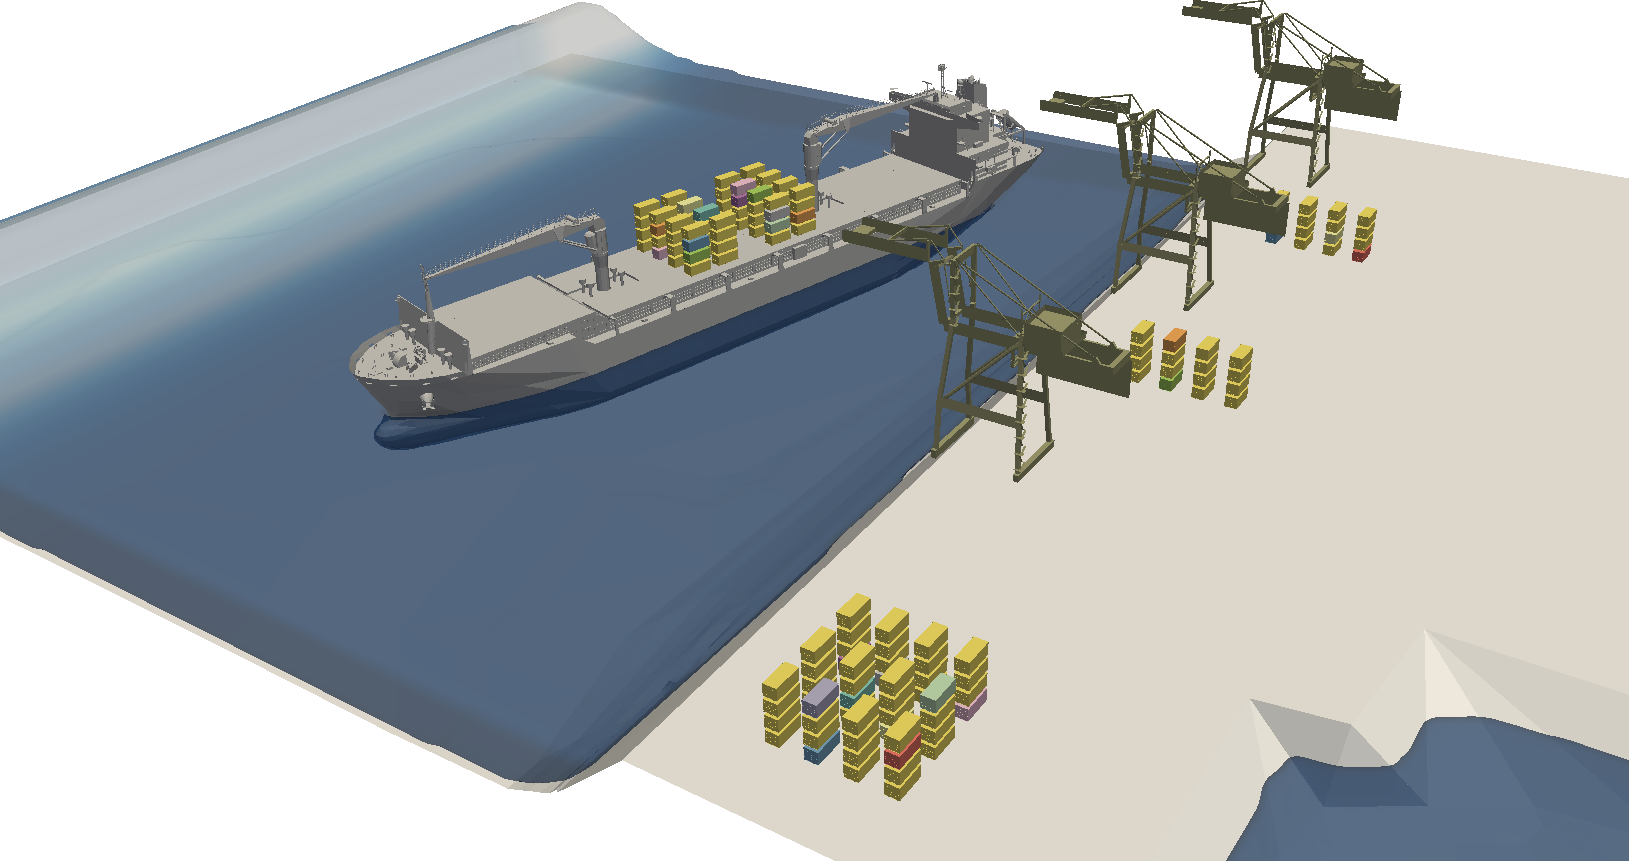
\includegraphics[width=0.95\linewidth]{Figures/6.Chapter/sines_ini_cond_II} 
	\caption{Initial conditions of the system.}
	\label{fig:sines_ini_cond} 
\end{figure}
%

The direction of the wave is normal to the quay wall structure. A cargo ship is placed in the domain, as well as a total of 143 ship containers, 64 of which on the ship. The ship has a density of $\rho=0.3\rho_{w}$ and the center of gravity was made to coincide with that of the actual ship. The geometry consists of the actual 3D scan of a ship hull, and was discretized as hollow, since no information on the internal structure of the ship is available and it would result in the most accurate inertia tensor. The ship containers are assumed half-full and as such with a $\rho=2.5\rho_{w}$ density. Each individual body has 6 degrees of freedom, no restrictions are applied, and are made of steel. The gantry cranes are also made of steel but are represented as fixed boundaries and the terrain was considered limestone. Table \ref{tab:material_props_sines} details the parameters used in the simulations. The \emph{CFL} constant was used as $C=0.2$, artificial viscosity with $\alpha=0.05$ and $h=\sqrt{3Dp^2}$.

%
\begin{table}[h]
\centering
\begin{tabular}{l|l|llll}
 & Material & $E\;[Nm^{-2}]$ & $\nu_p\;[-]$  & $e\;[-]$ & $\mu_f\;[-]$\\ \hline
Containers/Gantry cranes/Ship & Steel & $200\times10^9$ & $0.30$ & $0.85$ & $0.55$ \\
Terrain & Limestone & $4.5\times10^9$ & $0.15$ & $0.80$ & $0.60$
\end{tabular}
\caption{Young modulus, Poisson coefficient, restitution coefficient and friction coefficient used in the simulations.}
\label{tab:material_props_sines}
\end{table}
%

The wave travels approximately $7$ s until it hits the ship. The large acceleration immediately causes the instabilization of the most forward container stacks. Figure \ref{fig:sines_t38} represents the beginning of the ship motion and one can notice the beginning of the instabilization of the containers on the port-side.
\begin{figure}[H]
	\centering
	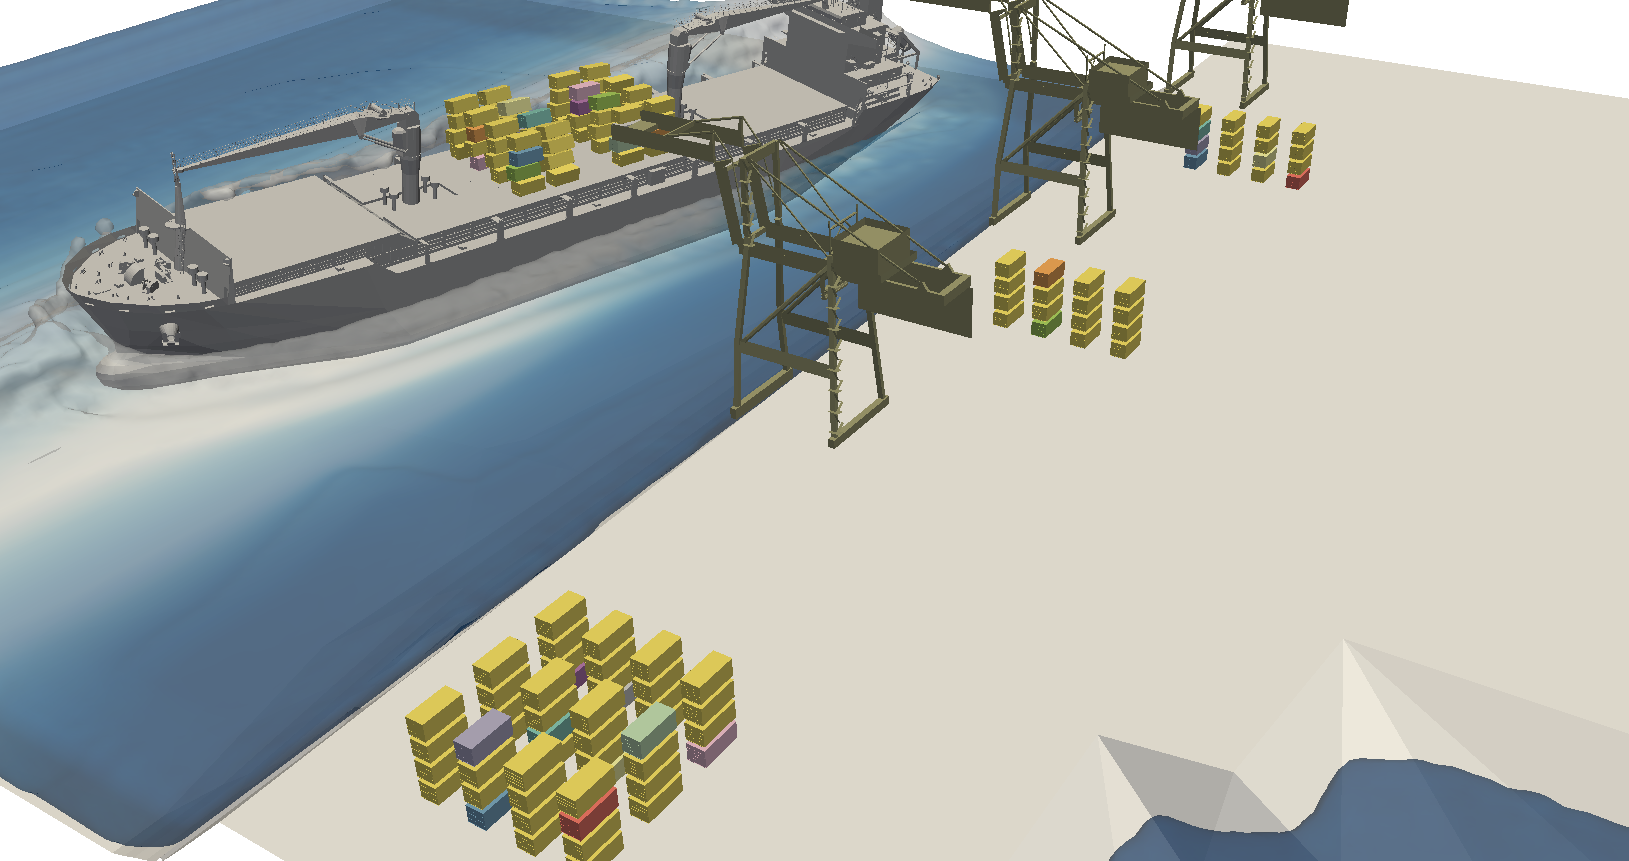
\includegraphics[width=0.95\linewidth]{Figures/6.Chapter/sines_t38_II} 
	\caption{General view of the application case, $t=7.6$ s.}
	\label{fig:sines_t38} 
\end{figure}
%

Figure \ref{fig:sines_t60}, at $t=12.0$ s, shows the container motion after the wave passage. 
\begin{figure}[H]
	\centering
	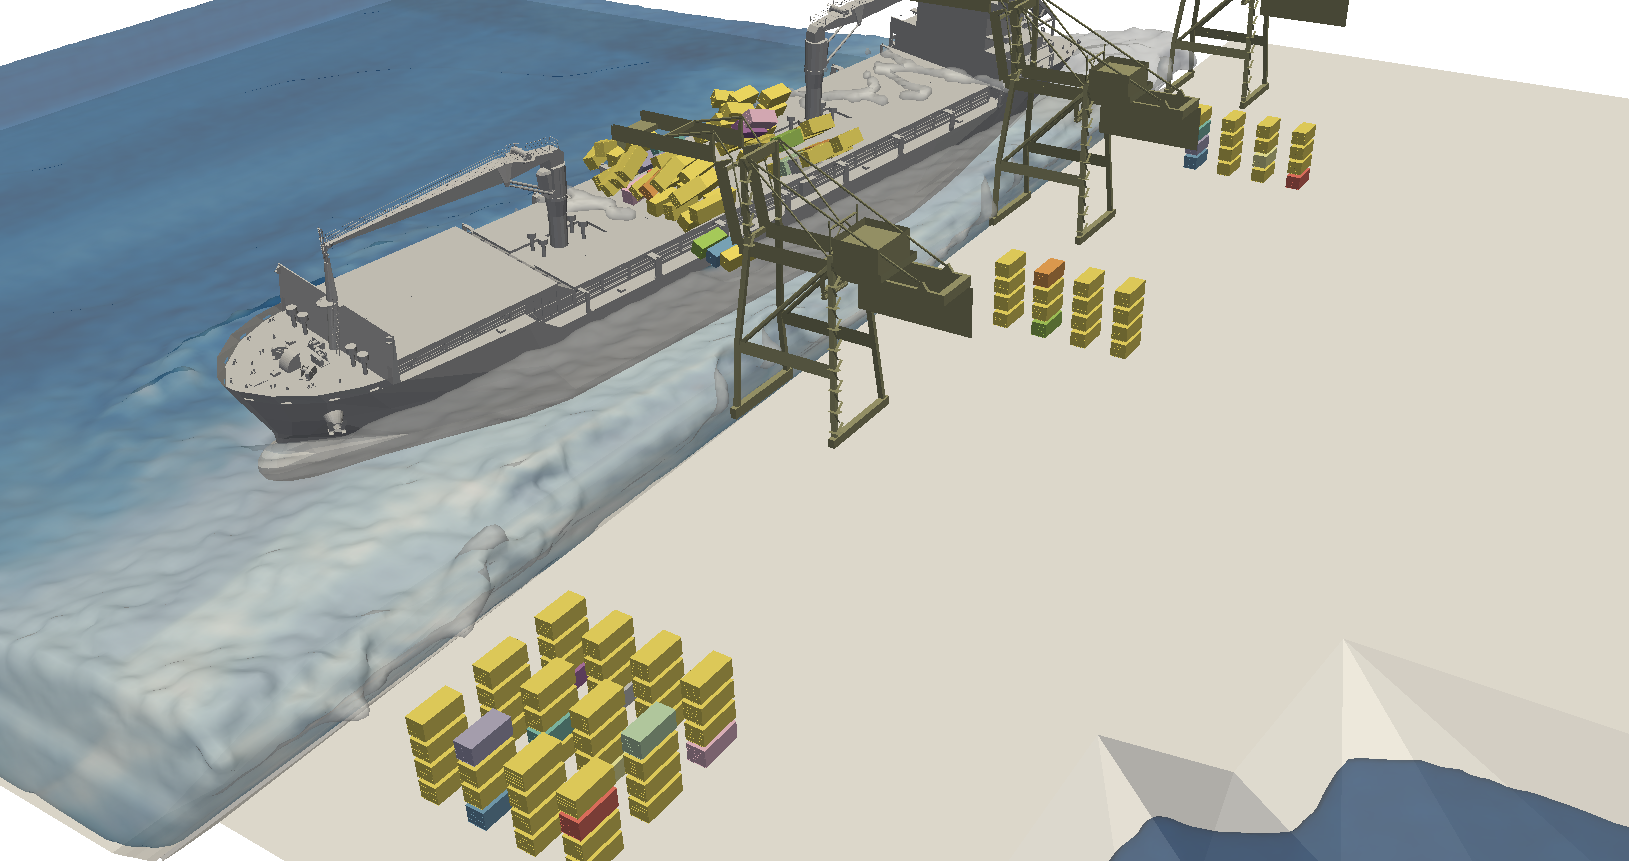
\includegraphics[width=0.95\linewidth]{Figures/6.Chapter/sines_t60_II} 
	\caption{General view of the application case, $t=12.0$ s.}
	\label{fig:sines_t60} 
\end{figure}
%

Figures \ref{fig:sines_t70} and \ref{fig:sines_t90}, at $t=14.0$ s and $t=18.0$ s, respectively, demonstrate the wave overtopping the quay and deforming at the base of the gantry cranes and the container stacks. 
\begin{figure}[H]
	\centering
	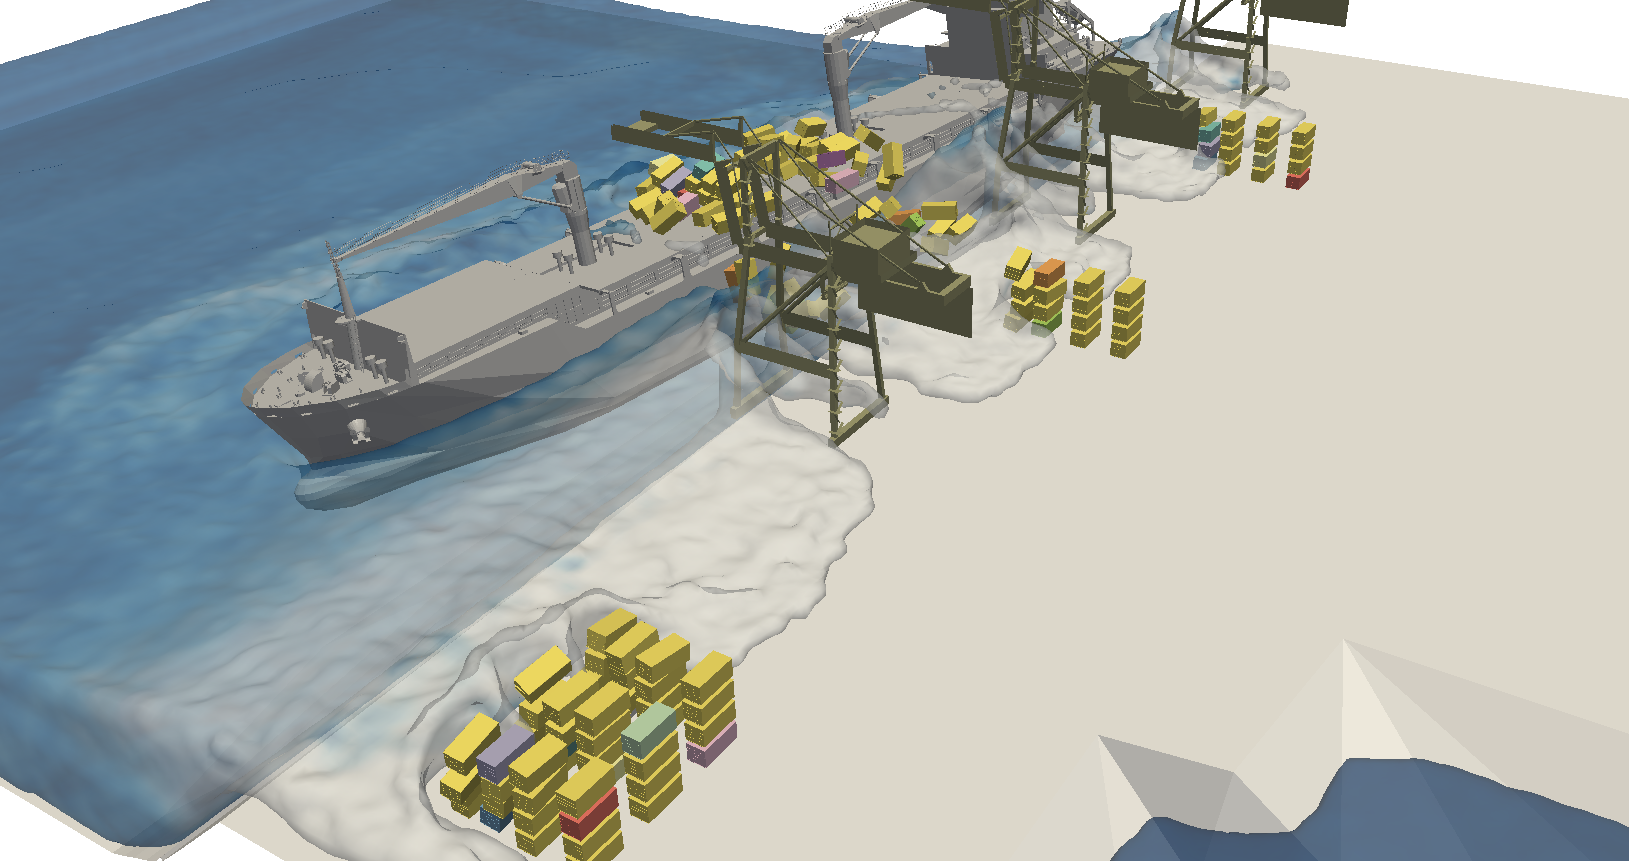
\includegraphics[width=0.95\linewidth]{Figures/6.Chapter/sines_t70_II} 
	\caption{General view of the application case, $t=14.0$ s.}
	\label{fig:sines_t70} 
\end{figure}
%
%
\begin{figure}[H]
	\centering
	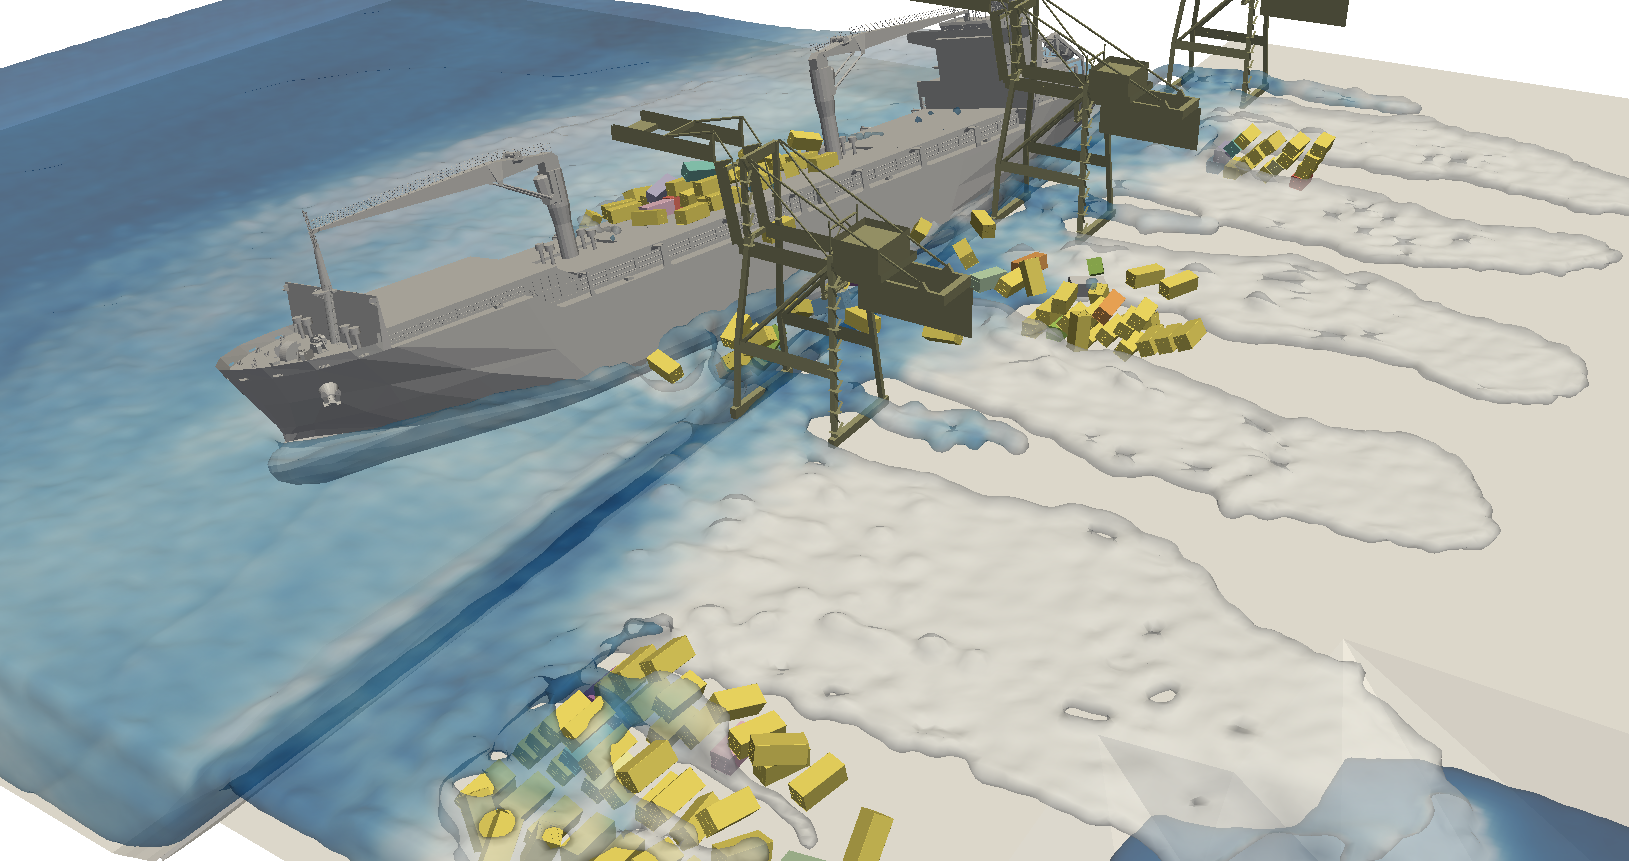
\includegraphics[width=0.95\linewidth]{Figures/6.Chapter/sines_t90_II} 
	\caption{General view of the application case, $t=18.0$ s.}
	\label{fig:sines_t90} 
\end{figure}
%
Instabilization of the piles is evident, with complex contact events being treated with no aberrant results. Containers initially aboard the ship are now in the water, most of them between the ship hull and the harbor structure.

Figure \ref{fig:sines_t300}, at $t=60.0$ s, show the state of the system at the end of simulated time.
\begin{figure}[H]
	\centering
	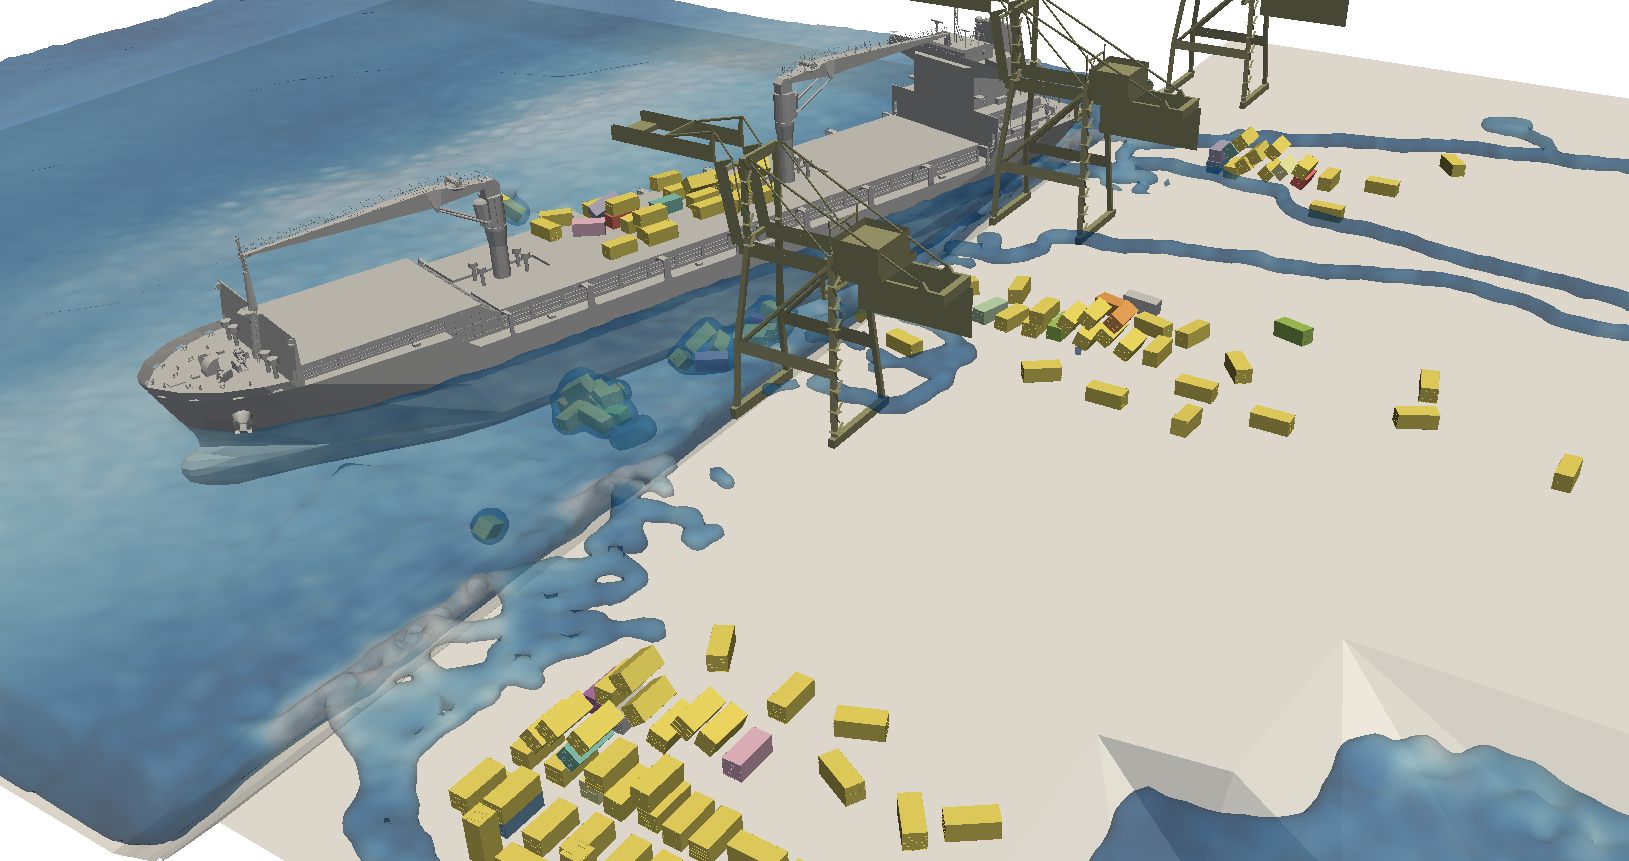
\includegraphics[width=0.95\linewidth]{Figures/6.Chapter/sines_t300_II} 
	\caption{General view of the application case, $t=60.0$ s.}
	\label{fig:sines_t300} 
\end{figure}
%
Some containers were dragged a considerable length, over $100\times$ its own characteristic dimensions. Large piles of containers can be seen, formed after the initial configurations were perturbed, since the wave did not have enough momentum to transport all the containers.

With a more detailed perspective over a set of containers, Figure \ref{fig:cont_t70}, at $t=14.0$ s, shows the instant immediately after wave impact. 
%
\begin{figure}[H]
	\centering
	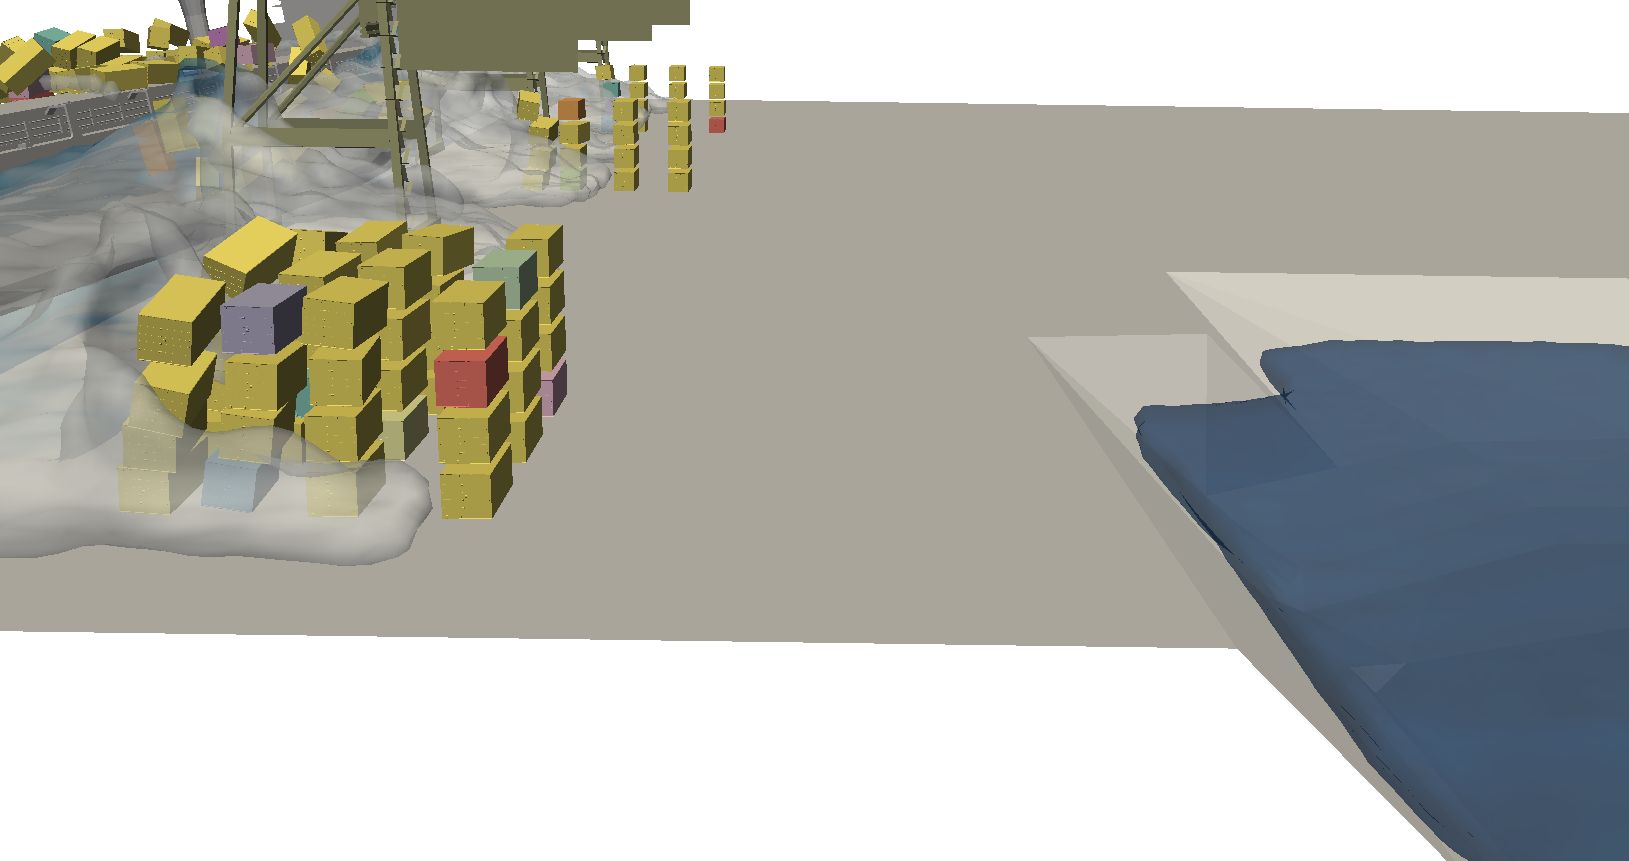
\includegraphics[width=0.95\linewidth]{Figures/6.Chapter/cont_t70} 
	\caption{Details of a set of container stacks, $t=14.0$ s.}
	\label{fig:cont_t70} 
\end{figure}
% 

Figures \ref{fig:cont_t80},\ref{fig:cont_t85} and \ref{fig:cont_t90} show the collapse of the set of containers due to the impact of the wave. Little motion of the containers is due to sustained transport, most of the momentum arises from the potential energy in the vertical pile and short contact forces due to the collisions. 
%
\begin{figure}[H]
	\centering
	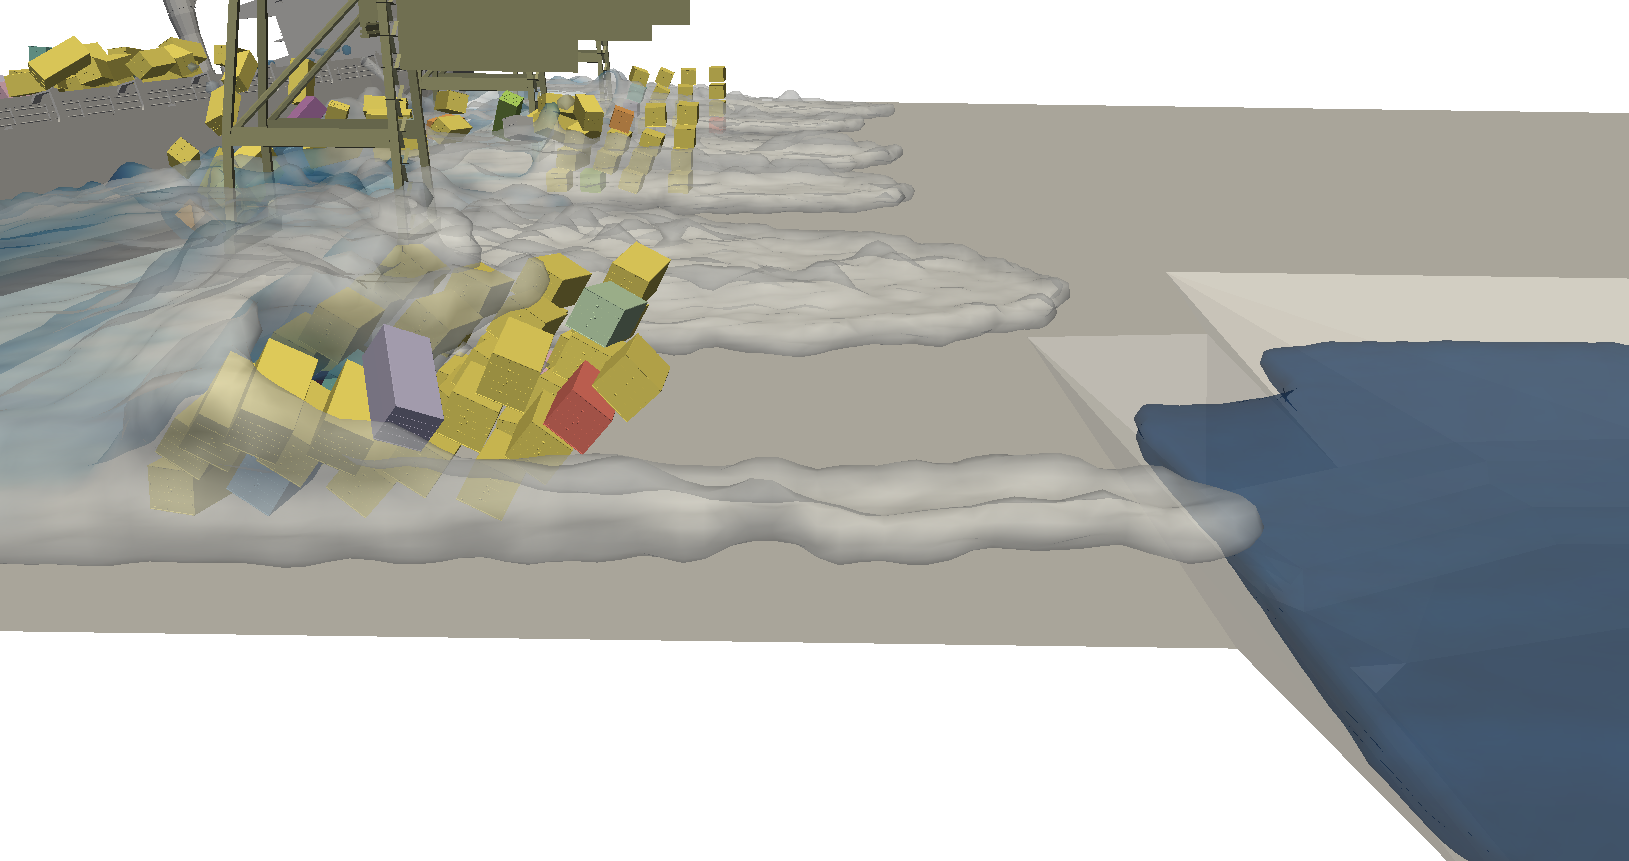
\includegraphics[width=0.95\linewidth]{Figures/6.Chapter/cont_t80} 
	\caption{Details of a set of container stacks, $t=16.0$ s.}
	\label{fig:cont_t80} 
\end{figure}
%
%
\begin{figure}[H]
	\centering
	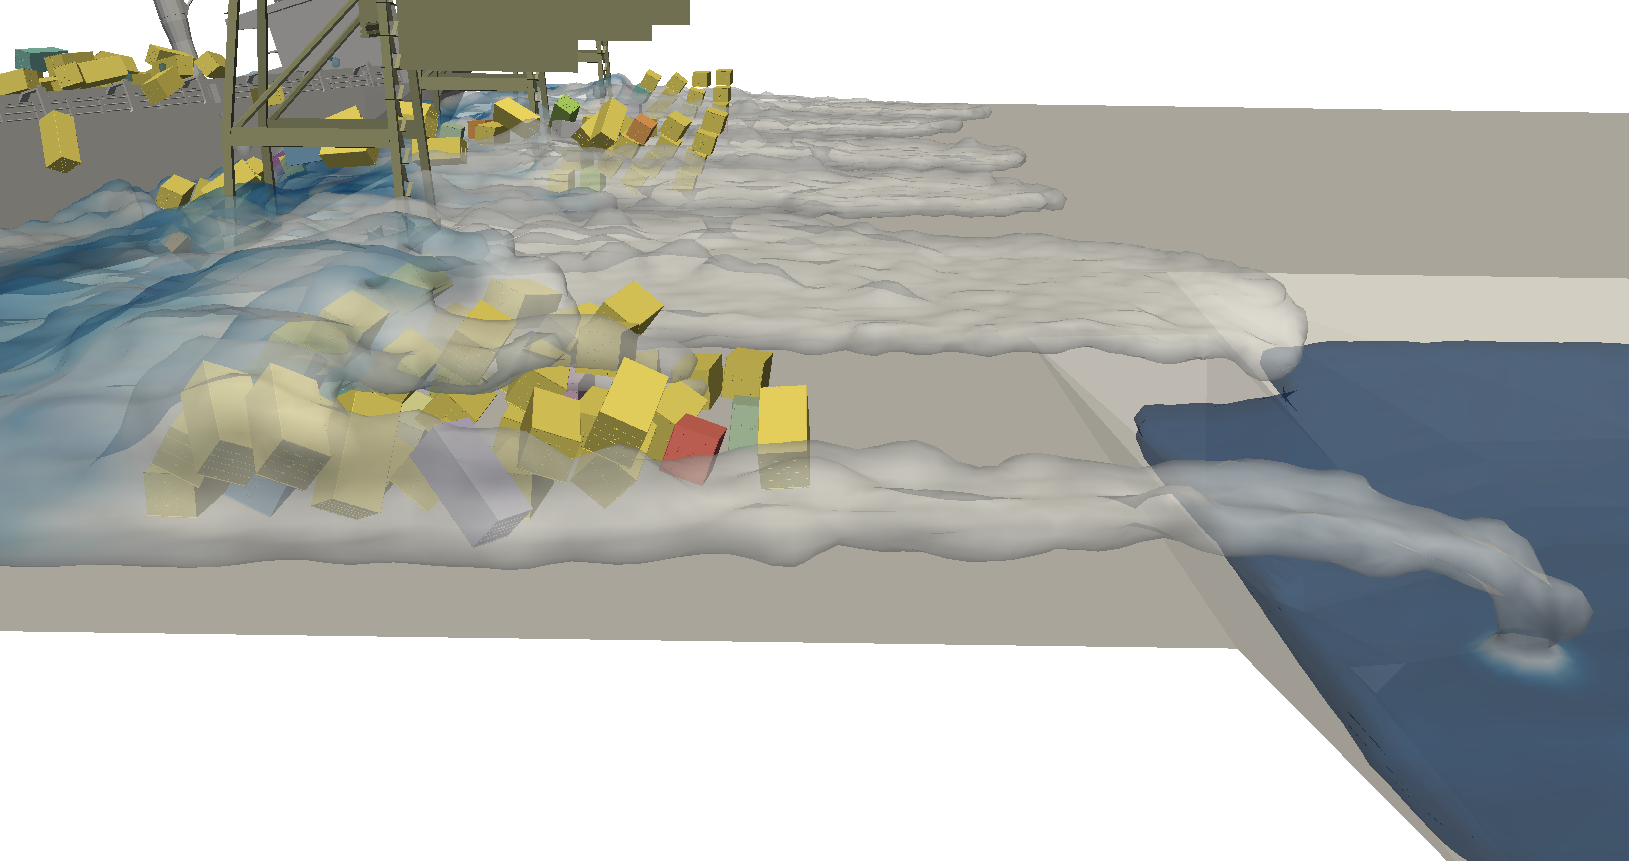
\includegraphics[width=0.95\linewidth]{Figures/6.Chapter/cont_t85} 
	\caption{Details of a set of container stacks, $t=17.0$ s.}
	\label{fig:cont_t85} 
\end{figure}
%
%
\begin{figure}[H]
	\centering
	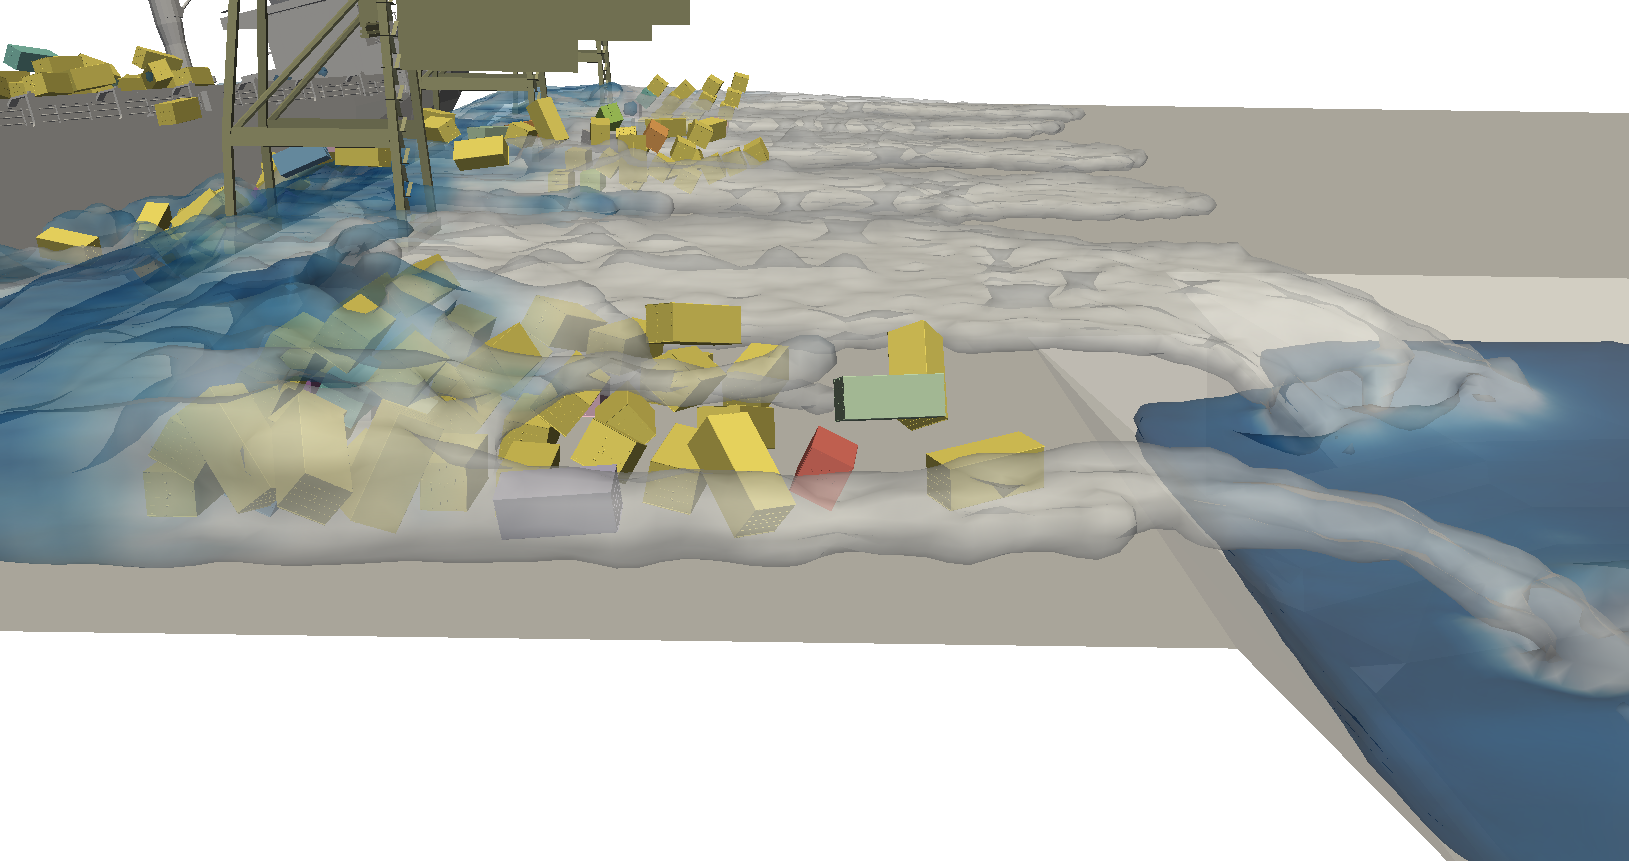
\includegraphics[width=0.95\linewidth]{Figures/6.Chapter/cont_t90} 
	\caption{Details of a set of container stacks, $t=18.0$ s.}
	\label{fig:cont_t90} 
\end{figure}
%

At $t=60.0$ s, Figure \ref{fig:cont_t300} shows the final set of the numerical solution. 
%
\begin{figure}[H]
	\centering
	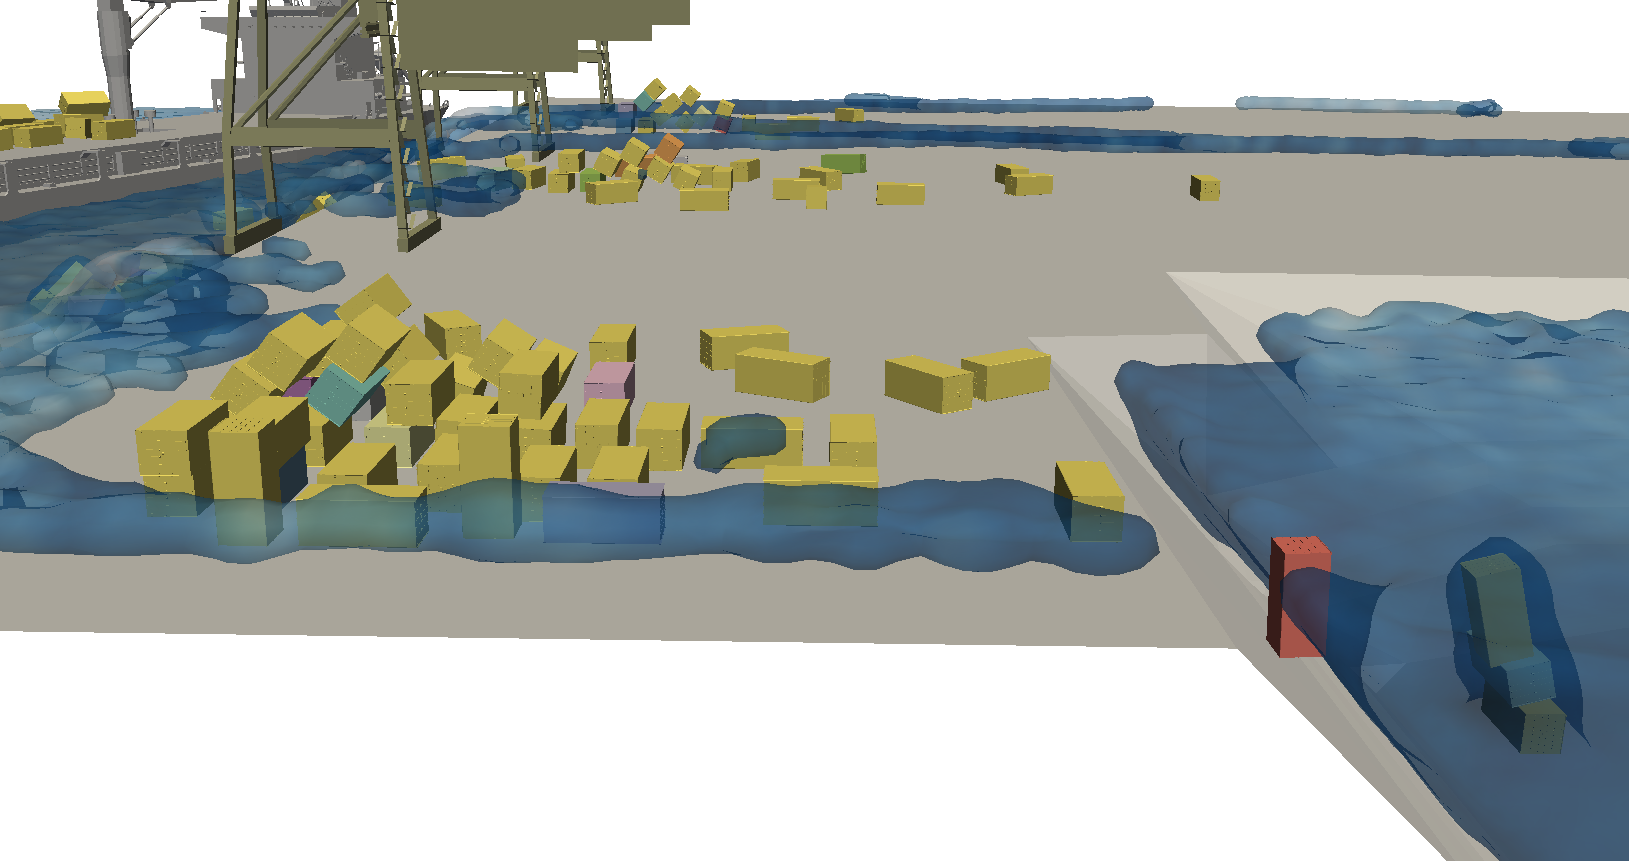
\includegraphics[width=0.95\linewidth]{Figures/6.Chapter/cont_t300} 
	\caption{Details of a set of container stacks, $t=60.0$ s.}
	\label{fig:cont_t300} 
\end{figure}
%
Some containers were projected across the structure platform but most did not incur in a significant dislocation. New equilibrium positions were achieved by the group of containers, showing the effectiveness of the contact mechanisms to provide balanced solutions even in complex configurations.

Focusing on the behavior of the ship containers aboard the ship, Figures \ref{fig:ship_t38} and \ref{fig:ship_t45} show the beginning of the instabilization as the wave passes, at $t=7.6$ s and $t=9.0$ s, respectively.
%
\begin{figure}[H]
	\centering
	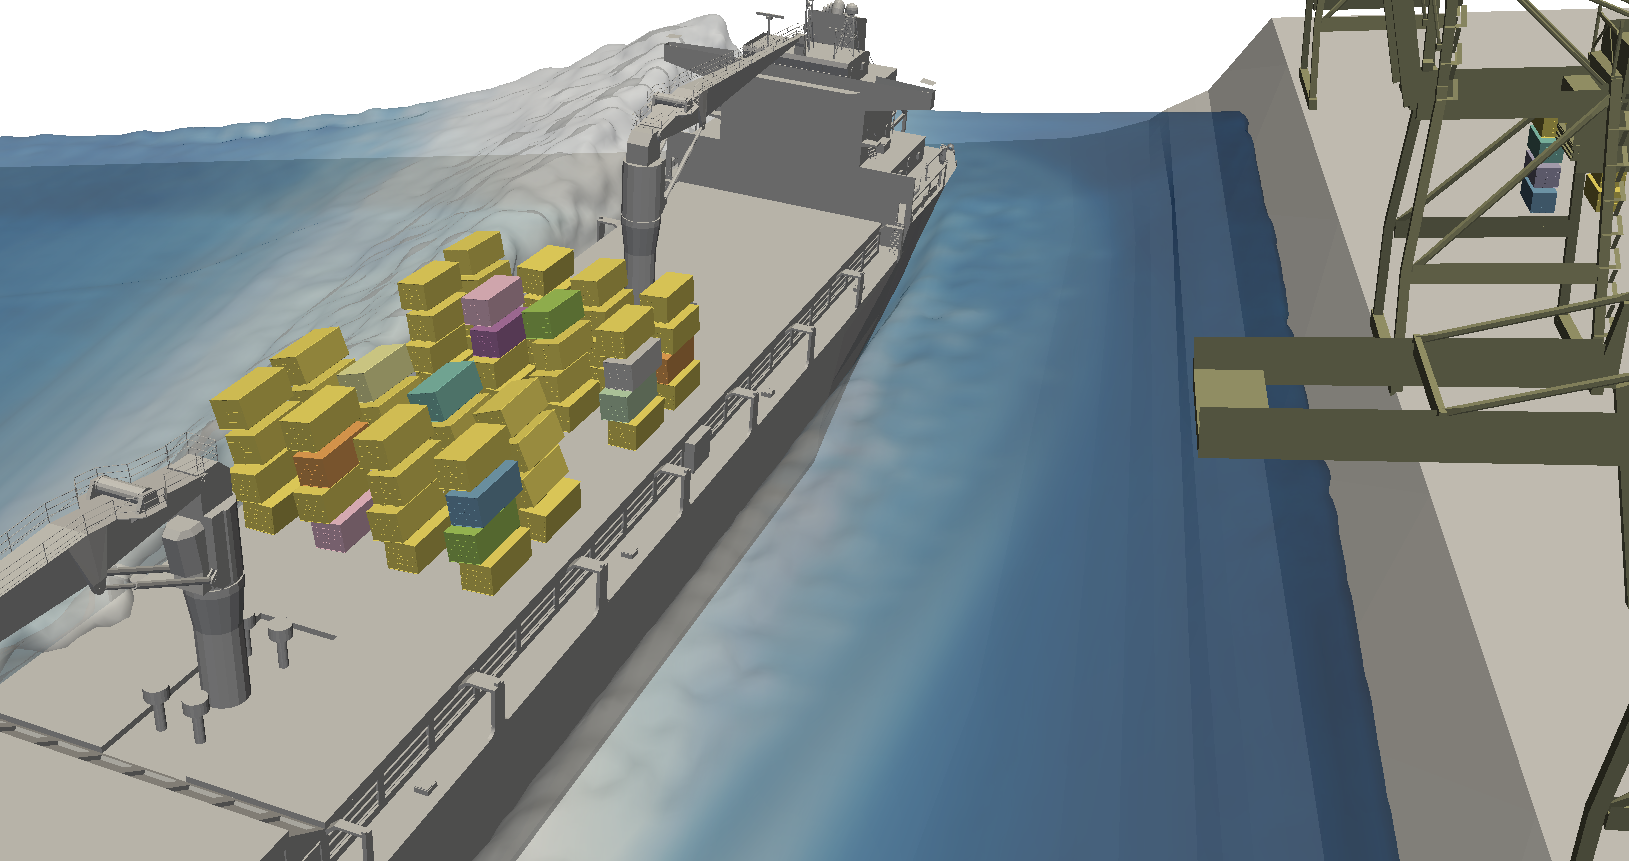
\includegraphics[width=0.95\linewidth]{Figures/6.Chapter/ship_t38} 
	\caption{Behavior of the ship-containers system, $t=7.6$ s.}
	\label{fig:ship_t38} 
\end{figure}
%
%
\begin{figure}[H]
	\centering
	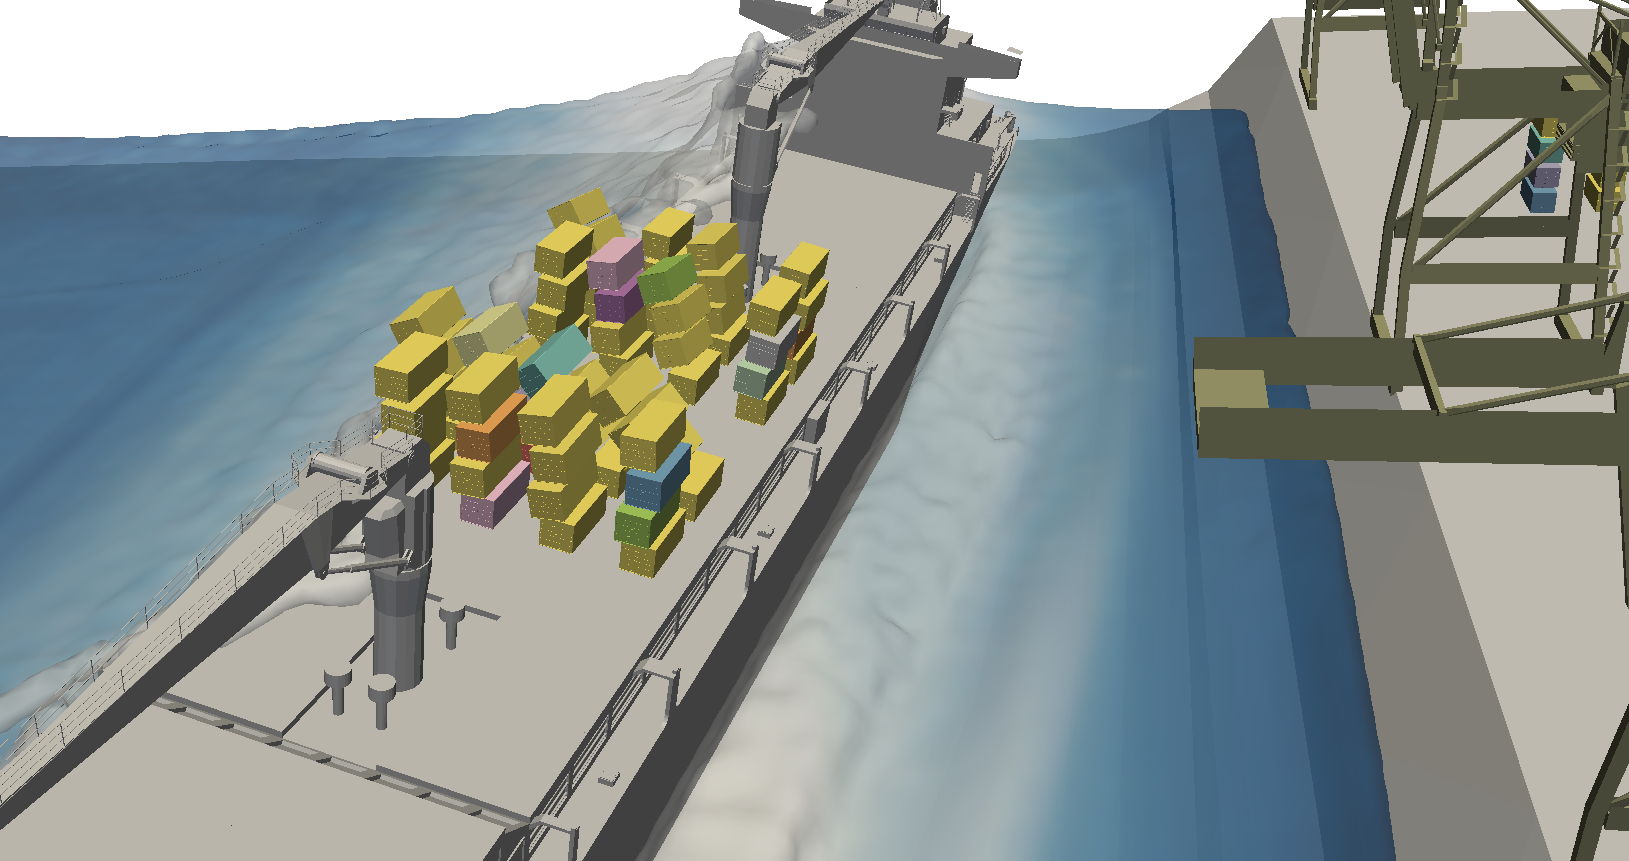
\includegraphics[width=0.95\linewidth]{Figures/6.Chapter/ship_t45} 
	\caption{Behavior of the ship-containers system, $t=9.0$ s.}
	\label{fig:ship_t45} 
\end{figure}
%

Figure \ref{fig:ship_t55} reflects the state of the system at $t=11.0$ s, were every set of containers is now in significant motion.
%
\begin{figure}[H]
	\centering
	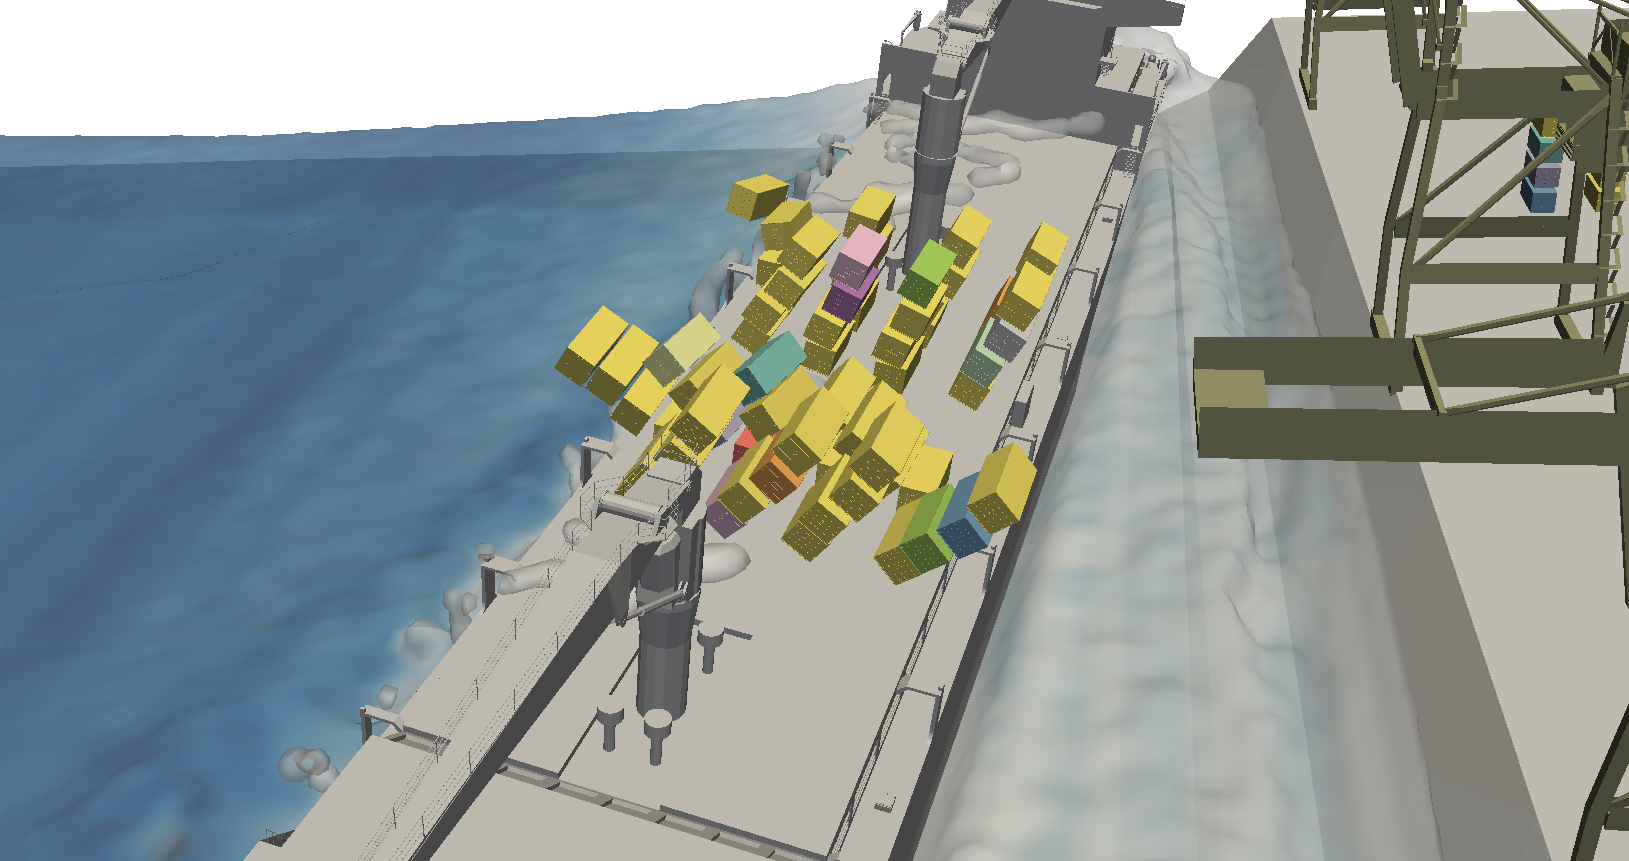
\includegraphics[width=0.95\linewidth]{Figures/6.Chapter/ship_t55} 
	\caption{Behavior of the ship-containers system, $t=11.0$ s.}
	\label{fig:ship_t55} 
\end{figure}
%

The uppermost containers are falling over the ship starboard-side, mostly due to inertia. The bottom containers, after being imprinted with the ship velocity by the friction mechanism, start sliding and falling port-side, as can be seen in Figure \ref{fig:ship_t65}. Such is due to the sudden acceleration of the ship caused by collision with the bottom and padding by the wave, now mostly between the ship and the harbor structure.
%
\begin{figure}[H]
	\centering
	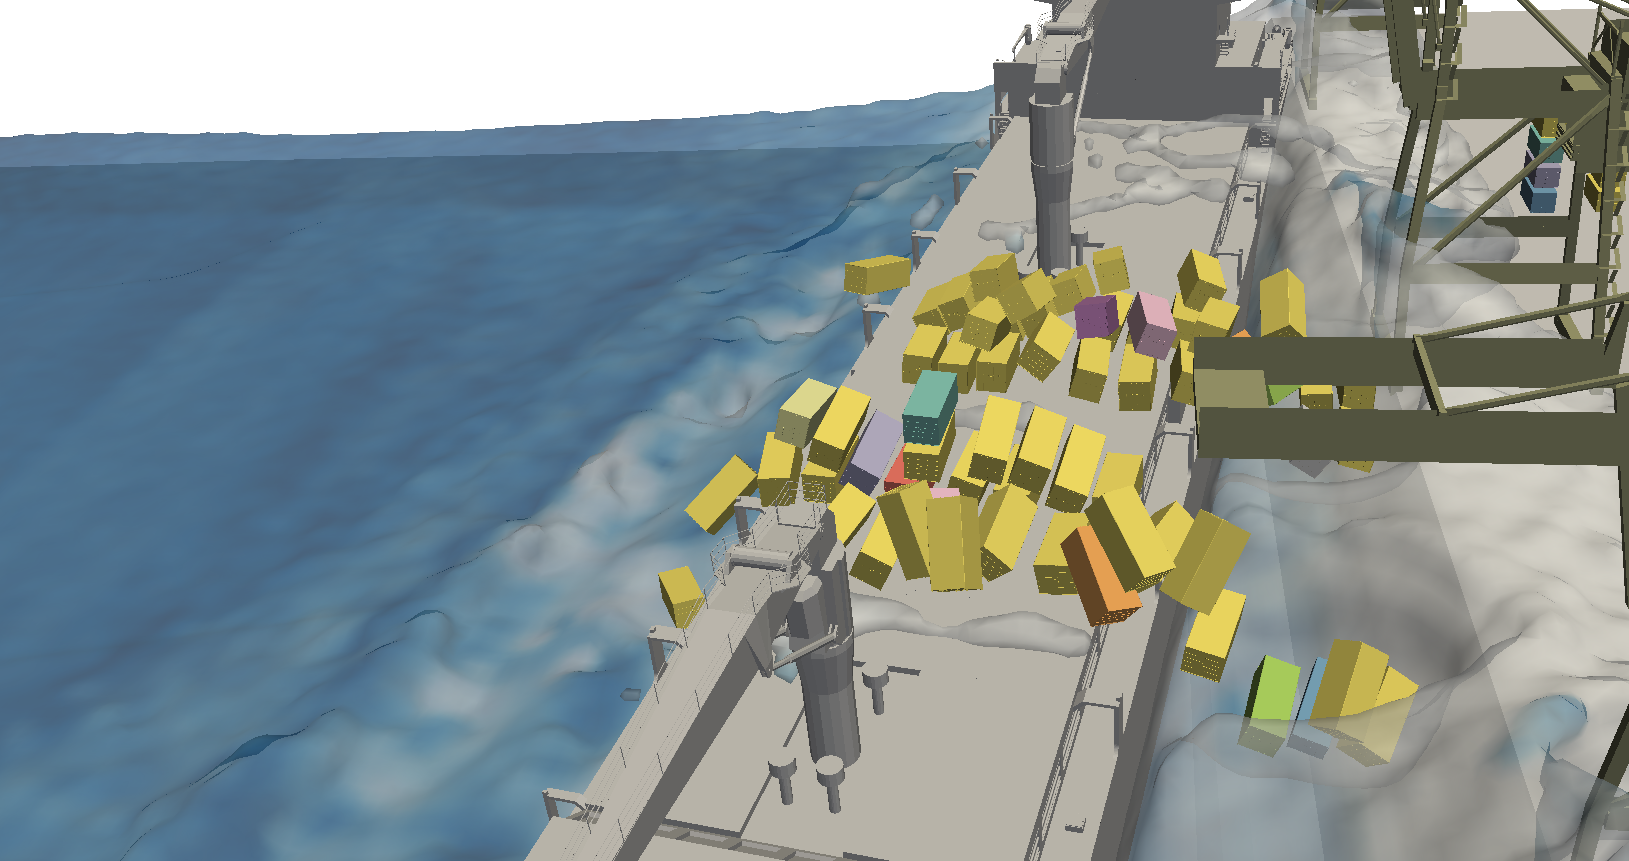
\includegraphics[width=0.95\linewidth]{Figures/6.Chapter/ship_t65} 
	\caption{Behavior of the ship-containers system, $t=13.0$ s.}
	\label{fig:ship_t65} 
\end{figure}
%

At the end of the simulation a considerable number of containers were transferred inland and a small amount fell overboard and are now in the fluid. The remaining containers have a solitary motion with the ship, as can be seen in Figure \ref{fig:ship_t300}, at $t=60.0$ s.
%
\begin{figure}[H]
	\centering
	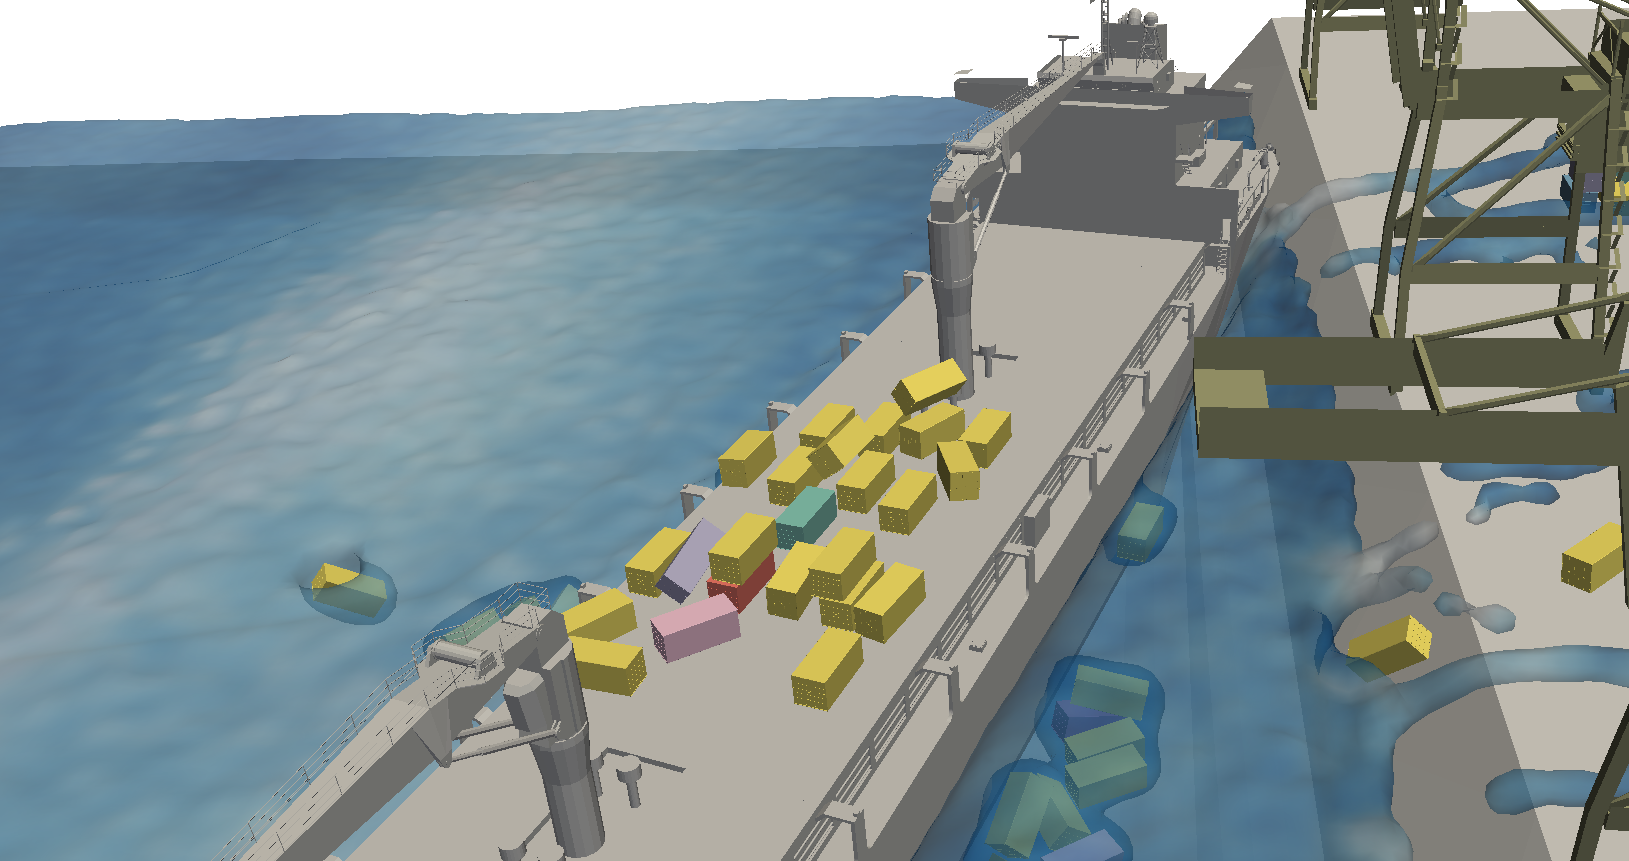
\includegraphics[width=0.95\linewidth]{Figures/6.Chapter/ship_t300} 
	\caption{Behavior of the ship-containers system, $t=60.0$ s.}
	\label{fig:ship_t300} 
\end{figure}
%


\clearpage
%%%%%%%%%%%%%%%%%%%%%%%%%%%%%%%%%%%%%%%%%%%%%%%%%%%%%%%%%%%
\section{Debris Flow}
\label{sec:debris_flow}

Debris flows are regarded as one of the most feared flow-related phenomena, due to the large destructive potential of infrastructure and danger to human lives. It is no surprise that a large body of work has been produced concerning its genesis, behavior and mitigation measures, both by fundamental phenomenological approaches reduced to analytic or simplified numerical problems and experimental campaigns. The flow characteristics ensure that complex measurements on important quantities remain difficult to perform. The inwards of a debris flow has only been accessible by analogy with simpler flows and conceptual work. Hope is therefore deposited in numerical work, to provide increasingly plausible insights into the mechanics of the flow. The amount of data amassed does not meet a reliable numerical solution, however. Existing conceptual models map poorly to a satisfactory numerical solution: the span of spacial scales involved in these flows start at the smaller energy carrying flow structures, up to the largest particles in the flow, possibly in the order of meters; the time scales range from millisecond inter-particle collisions to the duration of the flow; large deformations on the non-continuous multiphasic medium difficult any traditional approximation and the highly unsteady flow and free-surface deformations pose a challenge for state-of-the-art Finite-Volume codes, considering just single phase flows.

The application of the proposed model to a debris flow is done by reproducing an experimental campaign where debris flow mitigation measures are studied. A flume is fitted with a check-dam, intended to control the transport and deposition processes of the sediments carried downstream by debris flows. Since check-dams are considered as one of the simplest and most effective engineering measures against debris flows \citep{Zeng-2008,Remaitre-2008} they were widely applied all over the world as a short-term mitigation measure. Check dams are composed of a weir, two wings and a robust foundation, although there is a variety of other check dam solutions. Open-type check dams present a very attractive characteristic: they allow small sediment particles to pass through, while trapping larger blocks. The implemented open-type check dam is a slit dam, whose effectiveness in debris flows mitigation has been documented in the literature. 

The simulations are based on a flume described in \cite{Silva-2015}, where vertical slits with a spacing $s$, a $20\%$ slope and a recirculating mechanism are the main characteristics. The numerical flume presents fully periodic conditions, allowing for both fluid and solid phase recirculation. Two slit typologies were tested, named P1 and P2, as defined in \cite{Silva-2015}. Three spacings were tested, $s/d95 \in [1.18; 1.36; 1.49]$, as per the experiments. Figure \ref{fig:Slits} shows the dam section apparatus and defines the cross section of slits P1 and P2.

%
\begin{figure}[ht!]
	\centering
	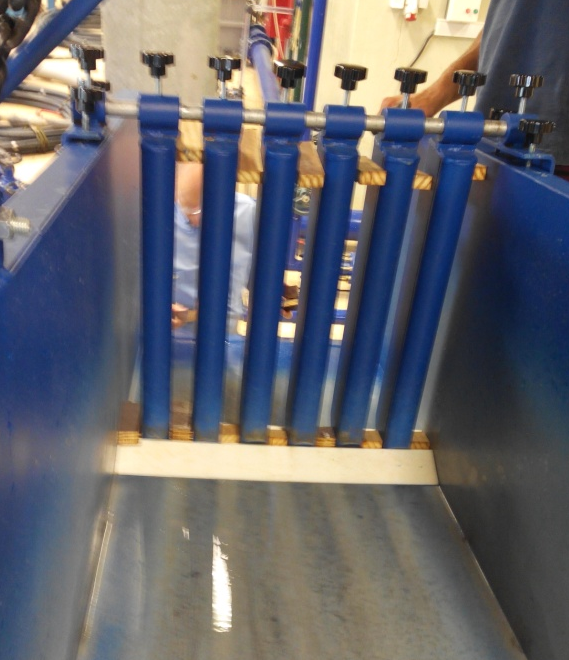
\includegraphics[width=0.45\linewidth]{Figures/6.Chapter/Experimental_slits}
	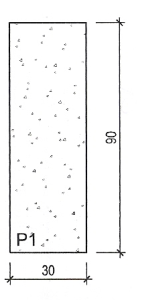
\includegraphics[width=0.20\linewidth]{Figures/6.Chapter/p1_slits}
	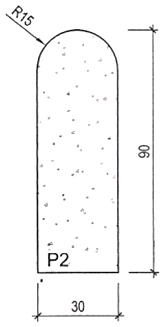
\includegraphics[width=0.205\linewidth]{Figures/6.Chapter/p2_slits}
	\caption{Experimental dam configuration. Slits P1 and P2 specifications. \citep{Silva-2015}}
	\label{fig:Slits} 
\end{figure}
%

The scales of the sediment grain interactions are orders of magnitude inferior to the $d50$ of the granulometric curve. This may represent a problem for the numerical discretization, as even smaller distances need to be evaluated for the force computations (Equation \eqref{eq:normal_viscoelastic_I}), and machine precision can start to affect the computations after a large number of iterations. In order to curb such effect, the geometric scale of the numerical experiment was doubled, as 

%
\begin{equation} \label{eq:Debris_scale_I}
	\lambda_l=\frac{L_m}{L_p}=2
\end{equation}
%
where $\lambda_l$ is the geometrical scale, $L_m$ is the characteristic length of the model and $L_p$ the same length on the physical prototype. Assuming Froude similarity, the discharge scales as
%
\begin{equation} \label{eq:Debris_scale_II}
	\lambda_Q=\frac{\lambda_V}{\lambda_t}=\frac{\lambda_l^3}{\lambda_l^{1/2}}=\lambda_l^{5/2}
\end{equation}
%

It is considered that liquid and solid discharges introduced upstream are independent, i.e., it is not intended that the solid discharge corresponds to the capacity discharge for the given liquid discharge, considering the inclination, geometry and roughness of the flume. Table \ref{tab:discharges} shows the used model discharges and the corresponding prototype values.

\begin{table}[!ht]
\begin{center}
\begin{tabular}{l|ll} 
 & Prototype & Model \\
\hline
$Q_l (m^3s^{-1})$ & 0.018 & 0.1018 \\
$Q_s (m^3s^{-1})$ & 0.00033 & 0.0018 
\end{tabular}
\end{center}
\caption{Model and prototype discharges}
\label{tab:discharges}
\end{table}

To promote a correct inlet of solid material, a hopper is modeled, placed on top of the channel. It was heuristically dimensioned to ensure an average solid discharge compatible with the one presented in Table \ref{tab:discharges}. 
Solid sediment grain sizes are generated according to a random algorithm that reproduces a log-normal function, effectively approximating the granulometric curve from \cite{Silva-2015}. The grains are dispersed in the hopper and are let to achieve their natural equilibrium positions at the start of the simulation. The initial conditions generation routines allows to create entirely distinct solutions based on the same granulometric curves, hence with comparable statistical properties, effectively corresponding to different experimental runs.

The proposed parameters for the material properties, used in Equations \eqref{eq:normal_viscoelastic_I} to \eqref{eq:elastic_fric}, are summarized in Table \ref{tab:materials}.

\begin{table}[!ht]
\begin{center}
\begin{tabular}{l|l} 
$E (GNm^{-2})$ & 45 \\
\hline
$\nu (-)$ & 0.35 \\
\hline
$\mu (-)$ & 0.35 
\end{tabular}
\end{center}
\caption{Sediment mechanical characteristics}
\label{tab:materials}
\end{table}

The resolution of the model was set at $0.008 \; m$, resulting in over $1.6\times10^6$ particles. 8 parallel simulations were carried out at a time on a Nvidia K20x cluster, each taking in excess of 280 h to model the 70 s runs, due to the very demanding stability constraints on time step. An overview of the domain can be seen in Figure \ref{fig:overall}.
%
\begin{figure}[ht!]
	\centering
	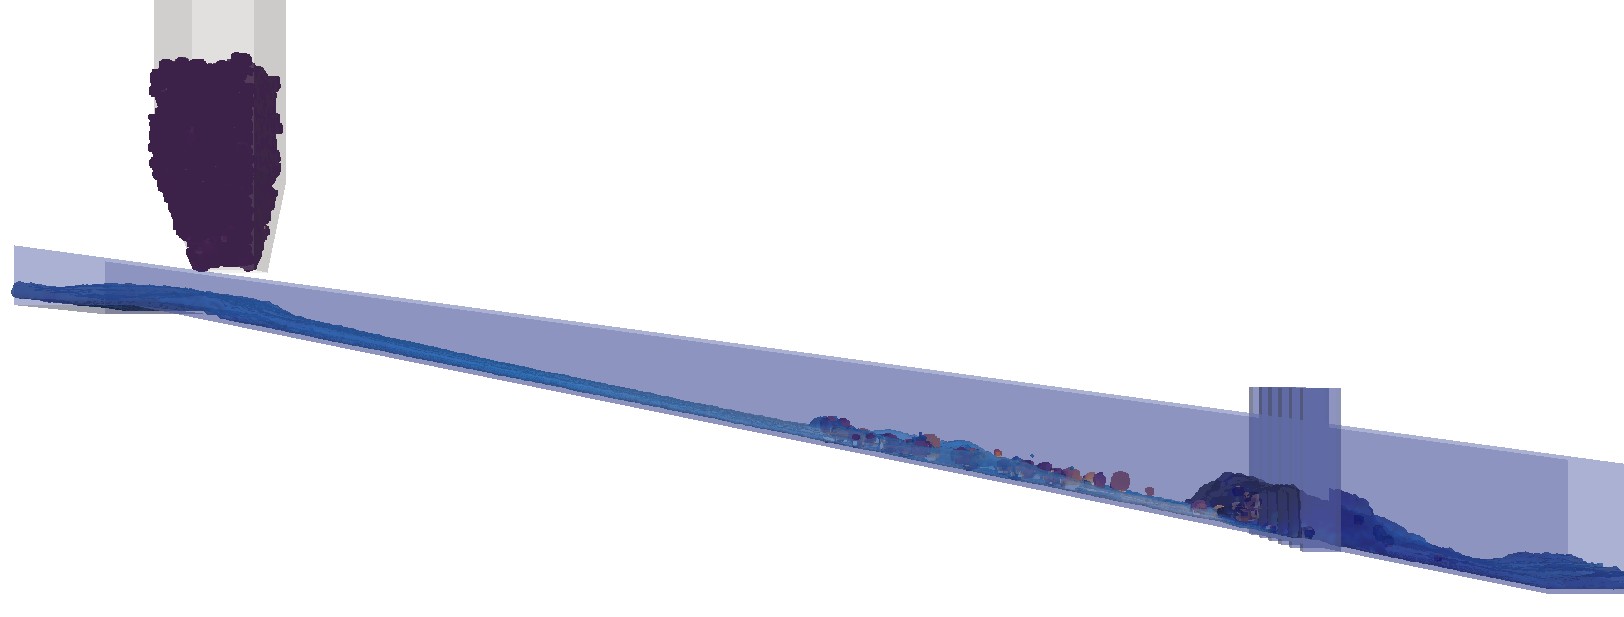
\includegraphics[width=0.75\linewidth]{Figures/6.Chapter/frame4}
	\caption{Overall domain configuration.}
	\label{fig:overall} 
\end{figure}
%

The sediment trapping efficiency is accounted by measuring the solid discharges at a position sufficiently upstream and immediately downstream of the dam. The experimental procedure estimated these by measuring the volumes of the sediment that was trapped downstream of the dam and by knowing the volume placed at the inlet. Due to the recirculation of solid particles, for the analysis of the numerical solution such approach is impractical, and discharges are computed directly by analyzing the flux of solid particles crossing a given plane.

Immediately after the opening of the hopper, a substantial amount of material falls to the flume, as indicated in Figure \ref{fig:t_2}, at $t=3.0$ s.
%
\begin{figure}[ht!]
	\centering
	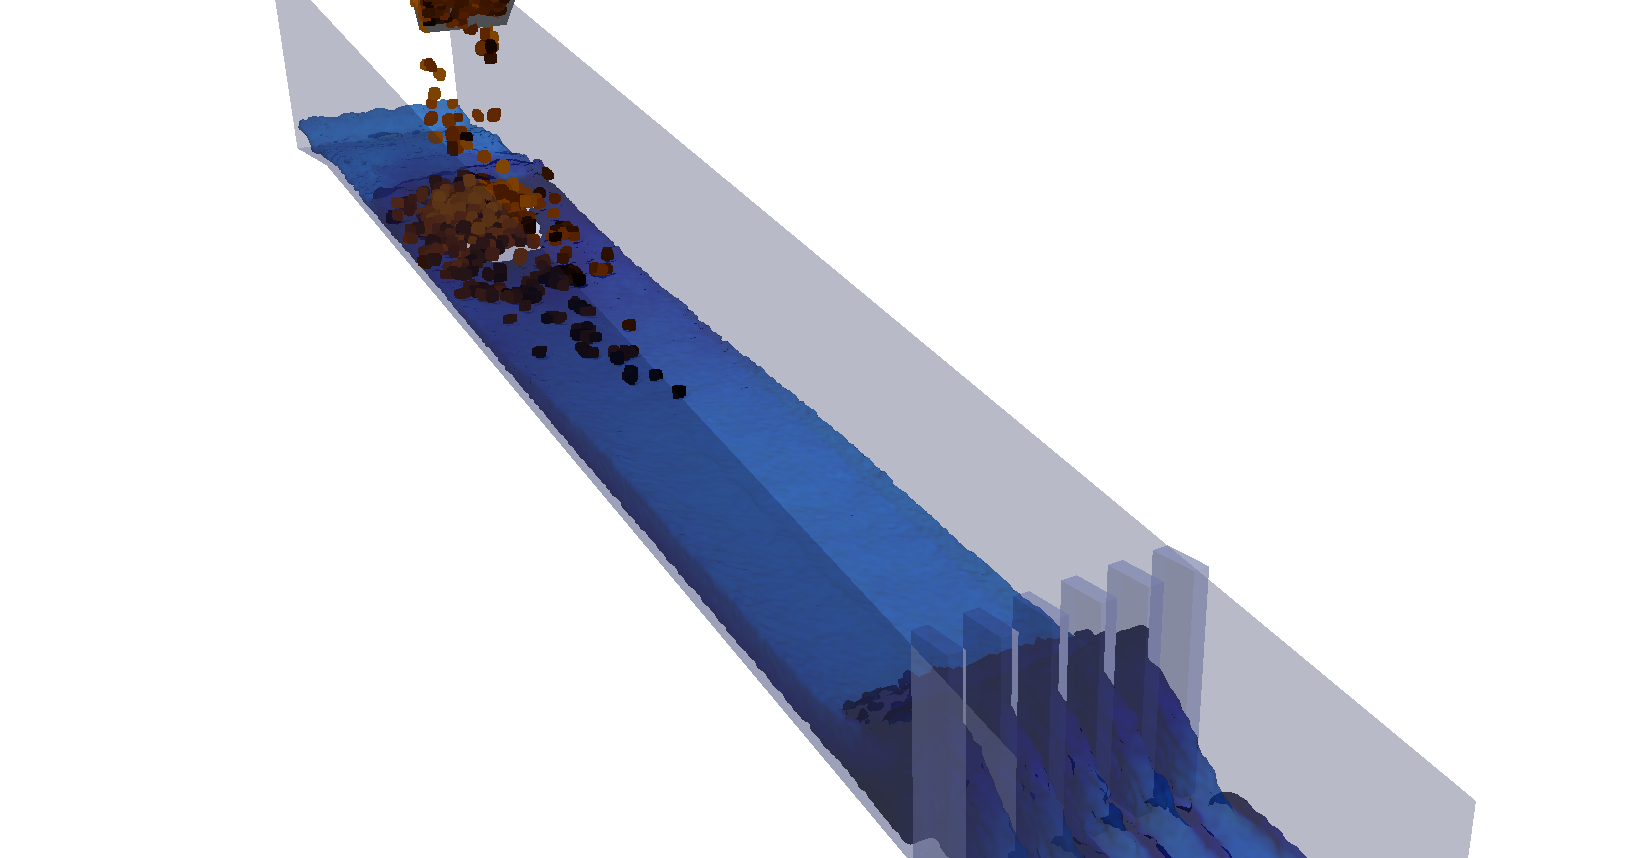
\includegraphics[width=0.75\linewidth]{Figures/6.Chapter/frame_II}
	\caption{P1 type slits, $t=3.0$ s}
	\label{fig:t_2} 
\end{figure}
%

As the material is carried downstream, deposition starts at the dam section. Figure \ref{fig:t_35} shows in detail a render of the solution in the dam area, at $t=8.0$ s.
%
\begin{figure}[ht!]
	\centering
	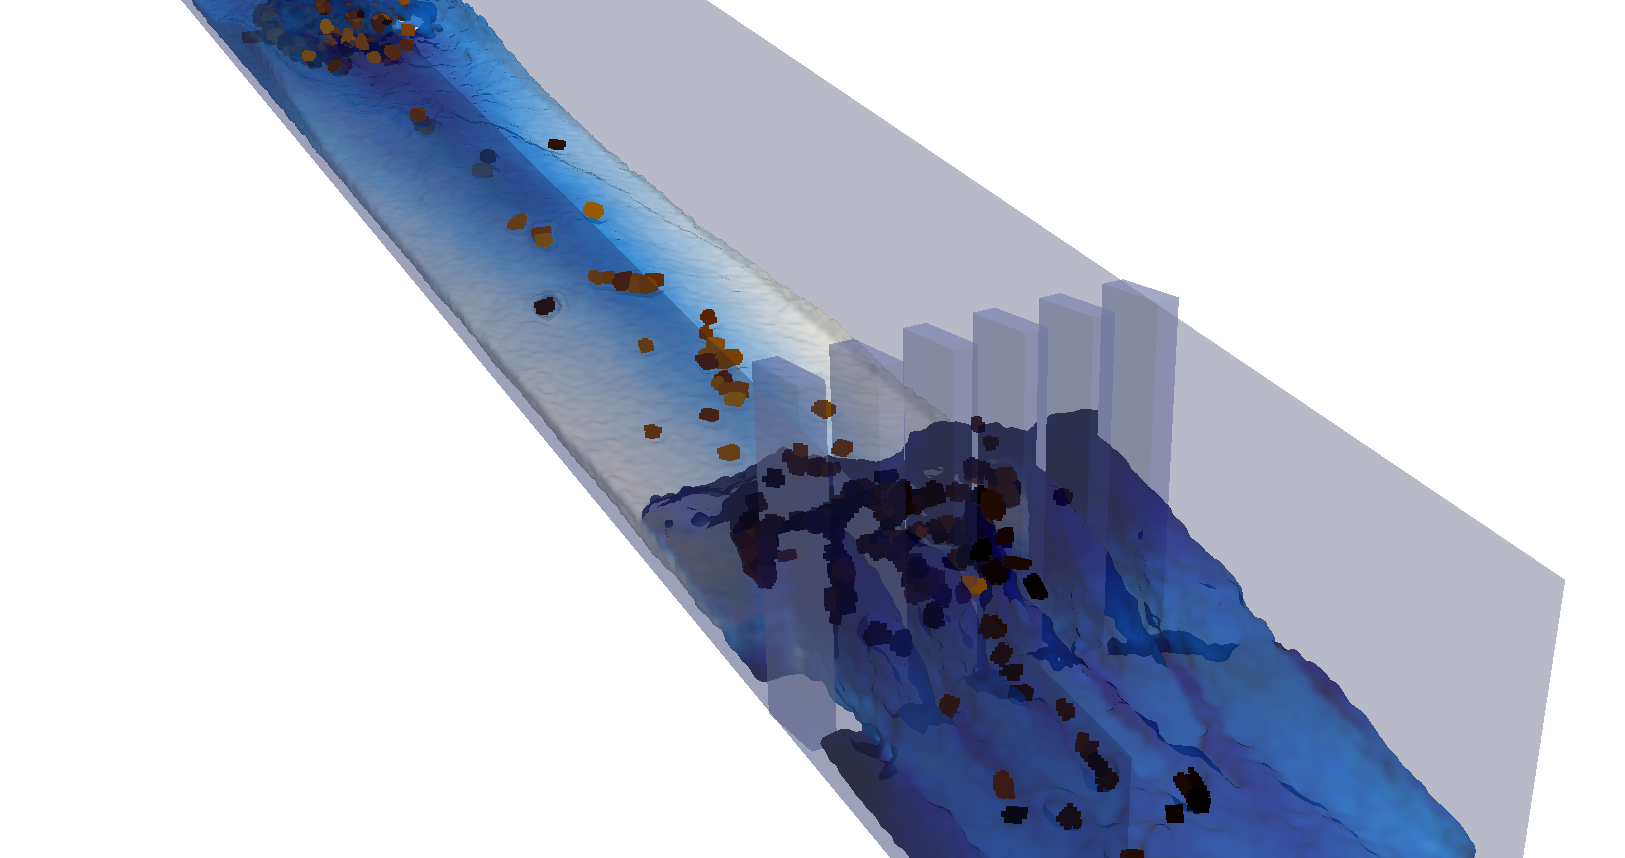
\includegraphics[width=0.75\linewidth]{Figures/6.Chapter/frame_V}
	\caption{P1 type slits, $t=8.0$ s}
	\label{fig:t_35} 
\end{figure}
%

As the material is dispensed from the hopper, the retention upstream of the dam becomes more effective. At $t=35.0$ s, the state of the solution is represented in Figure \ref{fig:t_350}. 
%
\begin{figure}[ht!]
	\centering
	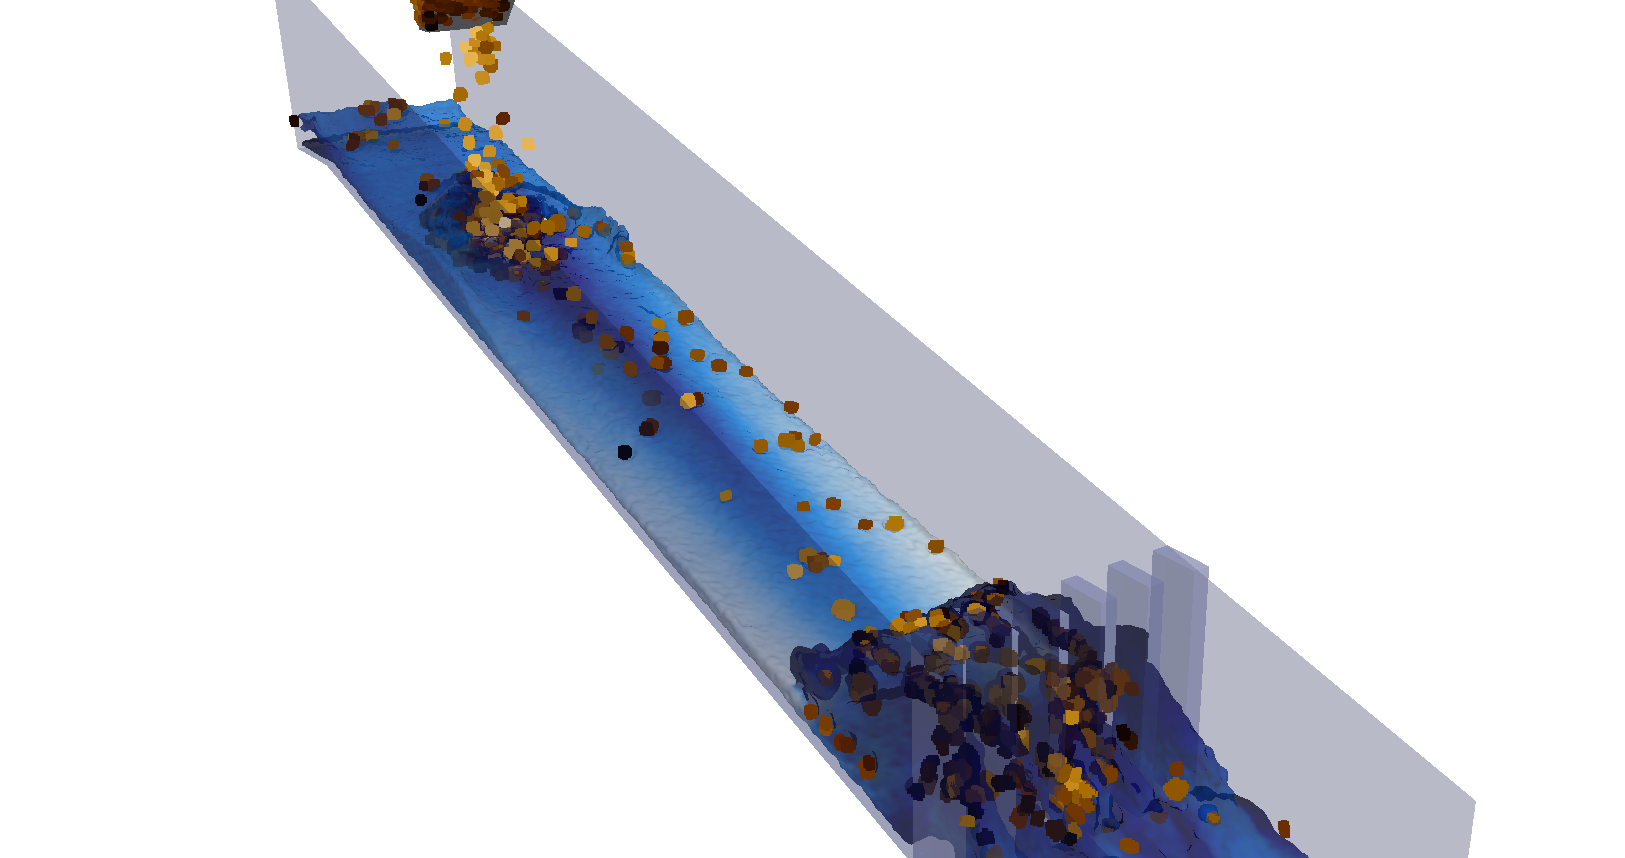
\includegraphics[width=0.75\linewidth]{Figures/6.Chapter/frame_III}
	\caption{P1 type slits, $t=35.0$ s}
	\label{fig:t_350} 
\end{figure}
%

Figures \ref{fig:t_2} to \ref{fig:t_350} are rendered from a particular simulation. As the sediment particles are generated with a random arrangement as initial conditions, significant instantaneous variations occur if one compares similar runs. On average, at $t=40.0$ s the hopper is exhausted and the flow is assumed to reach equilibrium conditions close to $10$ s after that, when the last solid particle reaches the backwater of the dam. A $15$ s interval was used to count solid discharges and derive retention trapping rates. Table \ref{tab:P1tr_comp} and Figure \ref{fig:P2tr_comp} show the relationship between sediment trapping efficiency, E, and the relative spacing $s/d95$ for each tested solution. 

\begin{table}[!ht]
\begin{center}
\begin{tabular}{l|llll} 
$s/d95$ & E[-] (Exp) & E[-] (Run I)& E[-] (Run II)& E[-] (Run III)\\
\hline
1.180 & 0.900 & 0.786 & 0.802 & 0.810 
\end{tabular}
\end{center}
\caption{Sediment trapping efficiency results. P1 type slits.}
\label{tab:P1tr_comp}
\end{table}

%
%\begin{figure}[ht!]
%	\centering
%	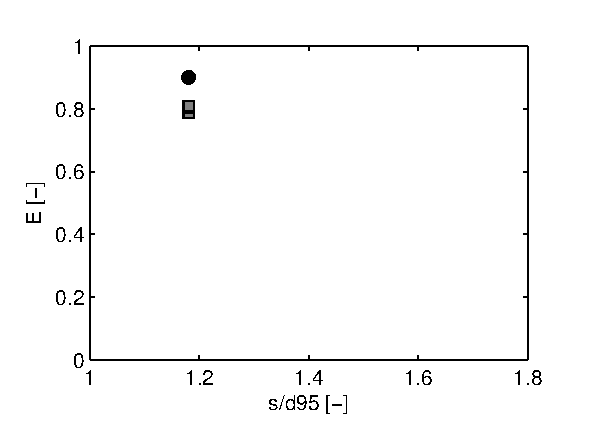
\includegraphics[width=0.50\linewidth]{Figures/6.Chapter/P1tr}
%	\caption{Sediment trapping efficiency results. P1 type slits. Experimental ($\cdot$) Numerical ($\square$)}
%	\label{fig:P1tr_comp} 
%\end{figure}
%

%
\begin{figure}[ht!]
	\centering
	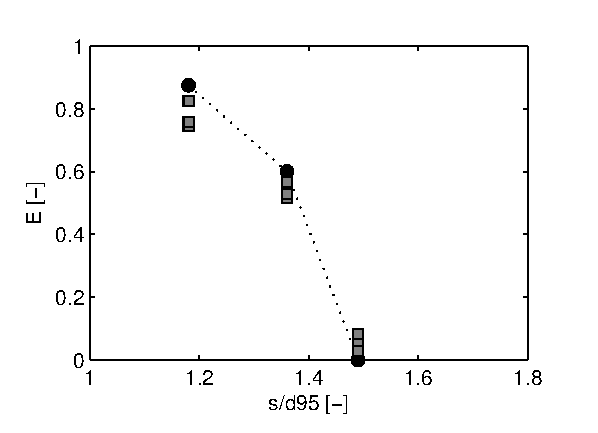
\includegraphics[width=0.50\linewidth]{Figures/6.Chapter/P2tr}
	\caption{Sediment trapping efficiency results. P2 type slits. Experimental ($\cdot$) Numerical ($\square$)}
	\label{fig:P2tr_comp} 
\end{figure}
%

The numerical results present a good comparison with the experimental data. A noticeable under prediction of the efficiency for small spacings is shown, for both slit geometries. For P2 slits the trend is accompanied with increasing spacing, but no zero efficiency is established for $s/d95=1.49$, contrasting with the experimental results. This is due to single sediment particles getting retained for long enough to affect the measurements on the numerical solution.

The differences should be explained both by discretization shortcomings and differences in the initial conditions from the experimental to numerical experiments. Besides conceptual considerations, the doubling of the geometrical dimensions to allow for more relaxed length and time scales is bound to introduce differences in the flow depth in the locus of the dam. This is because Froude similarity is not an exact hypothesis in the vicinity of the slits. This may affect the retention properties of the numerical dam, but insufficient experimental data is available to provide more insight. Another important difference is related to the initial conditions of the experimental procedure. These are not marked by a smooth, fixed bed: an approximately $5\;cm$ thick layer of sediment is deposited along the flume, also contributing to the total amount of mobile solid material if the flow is capable of mobilizing it, besides introducing considerable resistance to the flow.

The slit density, $\gamma_s$, is given by the ratio between the sum of all functional openings and the dam width, that influences water and solid discharges. Figure \ref{fig:SD_P1} shows the sediment trapping rate $E$ versus the slit density.

%
\begin{figure}[ht!]
	\centering
	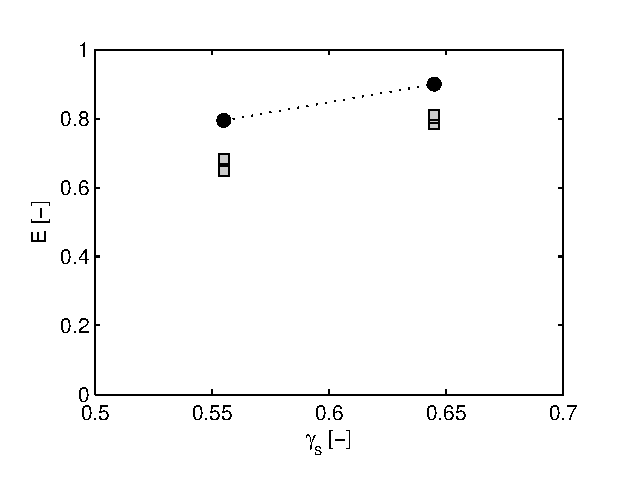
\includegraphics[width=0.50\linewidth]{Figures/6.Chapter/SD_P1}
	\caption{Sediment trapping rate as a function of slit density. P1 type slits for $s/d95=1.18$. Experimental ($\cdot$) Numerical ($\square$)}
	\label{fig:SD_P1} 
\end{figure}
%

An increase in slit density appears to induce increased efficiency of the solution, enhancing deposition upstream of the slit-dam. This is in line with the findings of \cite{Wenbing-2006}. For the same discharge, the average flow velocity decreases and the local stream power decreases too, resulting in the local reduction of sediment transport capacity. This effect seems to be captured in the numerical solution, albeit with the already discussed differences.







